\documentclass[11pt,a4paper]{article}
\usepackage[T1]{fontenc}
\usepackage[utf8]{inputenc}
\usepackage{lmodern,microtype}
\usepackage[margin=27mm,headheight=14pt]{geometry}
\usepackage{amsmath,amssymb,amsthm,mathtools}
\usepackage{booktabs,longtable,array,tabularx}
\usepackage{graphicx,xcolor,enumitem,fancyhdr}
\usepackage[hidelinks]{hyperref}
\usepackage[nameinlink,noabbrev]{cleveref}
\definecolor{ink}{RGB}{22,44,66}
\definecolor{accent}{RGB}{24,88,116}
\hypersetup{colorlinks=true,linkcolor=accent,citecolor=accent,urlcolor=accent,
pdftitle={Complex Transseries Reversion at Modular Cusps},
pdfauthor={Independent research study prepared with ChatGPT}}
\pagestyle{fancy}
\fancyhf{}
\fancyhead[L]{\small Complex transseries reversion}
\fancyhead[R]{\small Modular cusps and \(q\)-analogs}
\fancyfoot[C]{\thepage}
\setlength{\parskip}{4pt}
\setlength{\parindent}{1.2em}
\setlength{\emergencystretch}{2em}
\allowdisplaybreaks[2]
\setcounter{tocdepth}{2}
\numberwithin{equation}{section}
\newtheorem{theorem}{Theorem}[section]
\newtheorem{proposition}[theorem]{Proposition}
\newtheorem{lemma}[theorem]{Lemma}
\newtheorem{corollary}[theorem]{Corollary}
\newtheorem{definition}[theorem]{Definition}
\newtheorem{example}[theorem]{Example}
\newtheorem{remark}[theorem]{Remark}
\newtheorem{question}[theorem]{Research question}
\newcommand{\C}{\mathbb C}
\newcommand{\R}{\mathbb R}
\newcommand{\Z}{\mathbb Z}
\newcommand{\N}{\mathbb N}
\newcommand{\D}{\mathbb D}
\newcommand{\ii}{\mathrm i}
\newcommand{\ee}{\mathrm e}
\newcommand{\dd}{\,\mathrm d}
\newcommand{\Log}{\operatorname{Log}}
\newcommand{\Li}{\operatorname{Li}}
\newcommand{\Res}{\operatorname{Res}}
\newcommand{\ord}{\operatorname{ord}}
\newcommand{\lcm}{\operatorname{lcm}}
\newcommand{\sgn}{\operatorname{sgn}}
\newcommand{\Borel}{\mathcal B}
\newcommand{\Lap}{\mathcal L}
\newcommand{\bigO}{\mathcal O}
\newcommand{\coef}[2]{[#1^{#2}]}
\newcommand{\Poch}{P}
\newcommand{\repo}{\texttt{ProveIt}}
\newcommand{\sectors}{\mathcal S_\delta}
\begin{document}
\hypersetup{pageanchor=false}
\begin{titlepage}
\centering
\vspace*{8mm}
{\large\color{accent} RESEARCH ARTICLE\par}
\vspace{8mm}
{\Huge\bfseries\color{ink} Complex Transseries\\[2mm]
Reversion at Modular Cusps\par}
\vspace{8mm}
{\Large Stokes corrections, flat critical values,\\
arbitrary ramification, and \(q\)-gamma special values\par}
\vspace{8mm}
{\large An independent study of the \repo{} research questions\par}
\vspace{3mm}
{4 October 2026\par}
\vfill
\begin{minipage}{0.91\textwidth}
\begin{abstract}
Compositional inversion of a complex transseries requires a domain, a branch,
and a summation prescription.  We develop an explicit framework in which
those data remain visible throughout reversion, and apply it to
\(q\)-Pochhammer products at roots of unity.  First, an elementary
Mittag--Leffler calculation gives the meromorphic Borel transform of the
fixed-argument cyclotomic logarithm, all its poles and residues, uniform
Gevrey estimates, and its exact positive-ray Laplace sum.  A nonzero
residue correction disproves the unrestricted directional-equality clause
of the \repo{} conjecture \texttt{conj:cyclotomic-resurgent-inverse};
the appropriate replacement includes a specified summation direction
and Stokes corrections.  The resurgence itself is established literature,
which we explicitly identify.

Second, exact eta transformations reduce finite product quotients at every
rational cusp to an elementary exponential--power core times a convergent
series in a dual nome.  When the core cancels, we prove a convergent
logarithmic--Puiseux inverse, compute every coefficient, index all local
inverse sheets, and give an explicit truncation bound.  Three eta factors
realize every ramification order and are minimal for the two eta balances.
Four unnormalized Euler-product factors realize every ramification order
while cancelling all three perturbative balances; four are necessary.

Third, rational \(q\)-gamma special values have exact modular completions.
The half-argument completion is a theta function, whose lacunary series
yields an explicit logarithmic inverse.  For the original, unnormalized
\(q\)-gamma value we instead prove a regular-core inverse theorem with
sharp feedback scale \(t_0^{-2}\ee^{-S/t_0}\); its leading pole coefficients
are controlled by Lambert \(W\).  Exact rational calculations and high
precision complex checks accompany the proofs.  The results concern
specified formal or analytic classes and do not assert a global
inversion or summability theorem for unrestricted complex transseries.
\end{abstract}
\end{minipage}
\vfill
{\small Source comparison pinned to \repo{} commit\\
\texttt{6cb1d86f19ebf9f54c8d985b141b84233b6eab66}.}
\end{titlepage}
\pagenumbering{roman}
\hypersetup{pageanchor=true}
{\small\setlength{\parskip}{0pt}\tableofcontents}
\clearpage
\pagenumbering{arabic}
\section{Scope, results, and relation to the repository}\label{sec:scope}

In this article, \emph{series reversal} means \emph{compositional reversion}:
given a relation \(y=f(t)\), determine and justify a local inverse \(t=g(y)\).
It does not mean reversing the order of coefficients or taking \(1/f\).
The central issue is that an inverse may need a different asymptotic scale
from the original function.  The elementary example
\[
 y=\ee^{-S/t},\qquad
 t=-\frac{S}{\Log y+2\pi\ii j},\qquad j\in\Z,
\]
already exchanges an exponential scale for a logarithmic covering.
If the exponential is multiplied by a power of \(t\), Lambert \(W\)
enters.  If a leading correction is \(Q^m\), a Puiseux root enters before
the logarithm.  If the original coefficients are divergent, a choice of
Borel summation direction enters as well.

These mechanisms are often discussed separately.  Here they are joined in
an exact class arising from modular \(q\)-products.  The resulting theorems
include branch data and error bounds; they do not depend on promoting an
uncontrolled formal substitution to an analytic identity.

\subsection{What is proved}

The main results have five distinct roles.
\begin{enumerate}[leftmargin=*,itemsep=4pt]
\item \Cref{thm:cyclotomic-borel,thm:direction-counterexample} give an
explicit Borel transform for the fixed-argument cyclotomic \(q\)-Pochhammer
logarithm and a counterexample to one directional-equality assertion in
the repository.  The general resurgence mechanism is classical; the
point here is to state and prove the correctly normalized specialization.
\item \Cref{thm:core-inverse,thm:finite-endpoint} give two practical
reversion engines.  One treats an exact dominant core with a convergent
exponential tail.  The other treats a regular finite endpoint perturbed by
\(\ee^{-S/t}\), and identifies the sharp scale and all leading coefficient
poles.
\item \Cref{thm:cusp-normal-form,thm:flat-inverse} give the exact
normal form at every rational cusp and a convergent inverse when all
perturbative core terms cancel.
\item \Cref{thm:three-factors,thm:four-factors} construct arbitrary
finite ramification with minimal numbers of factors: three eta factors
for the two eta balances, four Euler-product factors for all three raw
product balances.
\item \Cref{thm:qgamma-completion} and the subsequent half-argument
calculation apply the theory to rational special values of \(q\)-gamma,
both before and after removal of their analytic background.
\end{enumerate}

A precise negative conclusion is part of the result:
a Borel ray containing no pole need not produce the same sum as another
such ray.  A precise positive conclusion is equally important:
after fixing the summation and logarithm sheets, an inverse can be
constructed with every exponential contribution retained and with a
geometric remainder.

\subsection{Existing results that must be credited}

The source comparison is pinned to commit
\texttt{6cb1d86f19ebf9f54c8d985b141b84233b6eab66}.
The \repo{} transseries volume and companion already contain exact-core
inversion, Lagrange--B\"urmann formulas, exponential corrections, and
positive-real \(q\)-product completions \cite{repo-trans,repo-companion}.
The support-controlled reversion and moving-fold reports already discuss
finite action grids, grouped resonances, and analytic critical charts
\cite{repo-reversion,repo-fold}.  The present argument does not claim
those principles as new.

The relevant source base also extends beyond the Transseries directory.
The \(q\)-Pochhammer monograph contains complex fixed-argument expansions,
cyclotomic asymptotic base inverses, exact eta completions at \(q=1,-1\),
ordinary finite ramification, and regular \(q\)-gamma base inversion
\cite{repo-qmono}.  It would therefore be incorrect to describe the
repository as confined to positive real \(q\).  Its frontier chapter
contains the named conjecture
\texttt{conj:cyclotomic-resurgent-inverse}, whose directional-equality
clause we test below.

The literature also goes substantially beyond a purely formal calculus.
Van der Hoeven proves formal compositional inversion in an appropriate
transseries field and develops a separate complex theory with
composition-domain restrictions \cite{vdh-book,vdh-complex}.
Edgar studies composition, recursion, and convergence
\cite{edgar}.  Marmi and Sauzin treat Borel transforms at roots-of-unity
resonances for a general cohomological equation
\cite[Sections 4.2--4.3]{marmi-sauzin}.  Their framework includes the
Lambert series used here.  Explicit quantum-dilogarithm Borel poles and
Stokes jumps are developed by Garoufalidis and Kashaev
\cite{garoufalidis-kashaev}; more recent \(q\)-Pochhammer modular
resurgence is treated by Fantini and Rella \cite{fantini-rella}.
Sauzin establishes nonlinear resurgent substitution and inversion under
the required analytic estimates \cite{sauzin}.

Our contribution is an explicit development within this established
framework: a correction of a specific repository assertion, exact
logarithmic cusp inversion with arithmetic coefficient generation,
sharp factor-count constructions, and the finite-endpoint feedback
analysis for modular \(q\)-gamma corrections.  These are proved below.
A worldwide priority claim, or the resolution of unrestricted complex
transseries inversion, would go beyond the evidence.

\subsection{Notation and domain conventions}

We use \(\N=\{0,1,2,\ldots\}\).  Put
\[
 P(z)=\prod_{n=1}^{\infty}(1-z^n),\qquad |z|<1.
\]
This is holomorphic and nonzero in the unit disk, and its logarithm is
the unique analytic logarithm with \(\log P(0)=0\).
The eta function is
\[
 \eta(\tau)=\ee^{\pi\ii\tau/12}P(\ee^{2\pi\ii\tau}),
 \qquad \Im\tau>0.
\]
For an integer \(n\ge1\), let
\(\sigma_{-1}(n)=\sum_{d\mid n}d^{-1}\).
A root of unity is written
\(\zeta=\ee^{2\pi\ii h/k}\), with \(k\ge1\) and \((h,k)=1\);
the cusp \(q=1\) is represented by \(h=0,k=1\).
We use
\[
 q=\zeta\ee^{-t},\qquad \Re t>0,\qquad
 \sectors=\{t:0<|t|<t_*,\ |\arg t|\le\pi/2-\delta\}.
\]
Here \(0<\delta<\pi/2\), and every asymptotic statement on
\(\sectors\) is uniform on the displayed closed subsector unless
explicitly qualified.

The symbol \(\Log\) denotes a specified branch or logarithm lift.
A logarithm of a holomorphic unit equal to \(1\) at the origin always
means its germ with value \(0\) there.  Thus a logarithm sheet is not
silently reset during continuation.  For complex \(q=\ee^{-t}\) and
rational \(x\), the definition of \(q^x\) is \(\ee^{-tx}\);
this is the branch used in the \(q\)-gamma applications.

\section{Complex reversion: formal data and analytic realization}
\label{sec:complex-framework}

\subsection{Three different meanings of a transseries inverse}

There are three levels of assertion.
A \emph{formal inverse} is an identity in a specified complete algebra
of series, where the relevant substitutions are defined.
An \emph{asymptotic inverse} is a sectorial function with controlled
remainders after truncation.
An \emph{exact convergent inverse representation} is an identity
obtained by substituting small functions into a convergent analytic
series.  Such a representation is stronger than its asymptotic expansion,
but does not supply all possible divergent or oscillatory transseries.

For example, if \(U(z_1,z_2)\) is analytic near \((0,0)\), then
\[
 U\bigl(\ee^{-\alpha/t},\ee^{-\beta/t}\bigr)
 =\sum_{p,q\ge0}u_{p,q}\ee^{-(p\alpha+q\beta)/t}
\]
converges whenever both arguments lie in a suitable polydisk.
It is an asymptotic transseries on a sector only when their real
exponential rates decay there.  If \(p\alpha+q\beta\) agrees for two
different pairs, their coefficients must be added before the leading
term is identified.  No denominator involving an action difference is
needed for this addition.

\begin{proposition}[Finite complex actions]\label{prop:finite-actions}
Let \(F(u,\mathbf z)\) be holomorphic near \((0,\mathbf0)\), with
\(F(0,\mathbf0)=0\) and \(F_u(0,\mathbf0)\ne0\).  There is a unique
holomorphic germ \(u=U(\mathbf z)\) with \(U(\mathbf0)=0\) and
\(F(U(\mathbf z),\mathbf z)=0\).
If \(z_j(t)=\ee^{-\alpha_j/t}\), and a closed sector satisfies
\[
 \Re(\alpha_j/t)\ge c/|t| \quad (1\le j\le r)
\]
for a fixed \(c>0\), then \(U(\mathbf z(t))\) is an exact convergent
sectorial transseries.  Its action support is contained in
\(\N\alpha_1+\cdots+\N\alpha_r\), and equal actions are grouped by
finite sums at each bounded exponential height.
\end{proposition}
\begin{proof}
The holomorphic implicit-function theorem gives \(U\) and a polydisk
of convergence.  Shrinking the sector radius puts all \(z_j(t)\)
in any smaller such polydisk.  Absolute convergence permits grouping.
On a fixed interior ray, the real part of
\(\sum n_j\alpha_j/t\), divided by \(1/|t|\), is at least
\(c\sum n_j\).  Consequently only finitely many multiindices lie below
a fixed height.  This proves both the finite grouping assertion and
the usual asymptotic interpretation of degree truncations.
\end{proof}

The finite-action result is standard analytic infrastructure.  It remains
useful because it says exactly which operation is legitimate.  An
arbitrary countable action family would additionally require control of
accumulation, coefficient summability, and substitution.  An arbitrary
complex direction may not meet a common decay cone at all.

\subsection{Why a global complex claim fails}

The size of \(\ee^{-1/t}\) changes when
\(\Re(1/t)\) changes sign.  The two functions
\[
 f_0(t)=t,\qquad f_1(t)=t+\ee^{-1/t}
\]
have the same algebraic asymptotic series on every closed right
subsector, but different inverses there.  Thus an algebraic expansion
does not determine exponentially small inverse information.
The exact normalizations in the following sections are what supply it.

A finite-point critical example is
\(f(t)=t^m\).  Its inverse requires an \(m\)-th root; it is not an
ordinary Taylor series at the critical value when \(m>1\).
At a flat cusp, \(\ee^{-1/t}\), even a Puiseux scale alone is
insufficient: a logarithm is unavoidable.
For arbitrary complex exponential actions, a sector may also contain
oscillatory pairs of comparable size.  A total real ordering of
monomials cannot simply be imported unchanged into that situation.
These distinctions are consistent with the composition restrictions
in the complex transseries literature \cite{vdh-complex}.

\subsection{A formal coefficient ring is not a summation theorem}

For coefficients in a complete formal algebra, an equation
\[
 u=-\Phi(u,\mathbf z),\qquad \Phi(0,\mathbf0)=0,
\]
with a suitably invertible linearization can be solved by coefficient
recursion.  In a \(\mathbf z\)-adic algebra, every coefficient uses
finitely many preceding coefficients.  That fact proves formal
existence and uniqueness.  It does not give bounds after substituting
a physical exponential scale.

For a resurgent extension, it is also insufficient that each
coefficient is individually resurgent.  An analytic series in a
second variable must have geometric coefficient bounds in the
relevant resurgent seminorms.  Sauzin's nonlinear implicit theorem
provides the appropriate setting \cite{sauzin}.  Our convergent
cusp theorems meet their analytic needs directly through ordinary
holomorphic estimates; our Borel calculations specify the
summation data rather than assuming it.


\section{Two quantitative reversion engines}\label{sec:engines}

\subsection{An exact core and all exponential coefficients}

Consider a function in a phase coordinate \(v\),
\begin{equation}\label{eq:core-form}
 F(v)=G(v)+L(\ee^{-\lambda v}),\qquad
 L(z)=\sum_{n\ge1}a_nz^n,
\end{equation}
where \(L\) is holomorphic at zero.
Choose a solution \(v_0\) of \(G(v_0)=w\), with \(G'(v_0)\ne0\).
The solution \(v_0\) is a \emph{chosen core branch}; the theorem below
does not claim that the core is globally one-to-one.

Define its divided difference
\[
 D_{v_0}(u)=
 \begin{cases}
 (G(v_0+u)-G(v_0))/u,&u\ne0,\\
 G'(v_0),&u=0.
 \end{cases}
\]
It is holomorphic wherever the translated core is holomorphic.
Writing \(v=v_0+u\), \(\xi=\ee^{-\lambda v_0}\), converts the
inverse equation exactly to
\begin{equation}\label{eq:core-implicit}
 u+\frac{L(\xi\ee^{-\lambda u})}{D_{v_0}(u)}=0.
\end{equation}

\begin{theorem}[Exact-core reversion]\label{thm:core-inverse}
Suppose \(D_{v_0}\) is holomorphic and nonzero on a neighborhood of
\(|u|\le r\), and for some \(\rho>0\), \(0<\kappa<1\),
\[
 \left|\frac{L(z\ee^{-\lambda u})}{D_{v_0}(u)}\right|
 \le\kappa r
 \qquad (|u|\le r,\ |z|\le\rho).
\]
The equation has one simple root \(u=U(v_0,z)\) in \(|u|<r\),
holomorphic in \(z\) and any holomorphic core parameters.  It has a
convergent expansion
\[
 U(v_0,z)=\sum_{n\ge1}U_n(v_0)z^n.
\]
Put \(a_n^{(j)}=[z^n]L(z)^j\).  Every coefficient is
\begin{equation}\label{eq:all-core-coefficients}
 U_n(v_0)=
 \sum_{j=1}^n\frac{(-1)^j a_n^{(j)}}{j!}
 \left.
 \frac{\mathrm d^{j-1}}{\mathrm du^{j-1}}
 \left(\frac{\ee^{-n\lambda u}}{D_{v_0}(u)^j}\right)
 \right|_{u=0}.
\end{equation}
For \(\eta=|z|/\rho<1\), the tail after degree \(N\) satisfies
\begin{equation}\label{eq:core-tail}
 \left|U(v_0,z)-\sum_{n=1}^NU_n(v_0)z^n\right|
 \le \frac{\kappa r\,\eta^{N+1}}{1-\eta}.
\end{equation}
\end{theorem}
\begin{proof}
On \(|u|=r\), the second term of \cref{eq:core-implicit} is
strictly smaller than \(u\).  Rouch\'e's theorem counts exactly one
zero, with multiplicity.  It is therefore simple.
The holomorphic implicit-function theorem gives its local analytic
dependence; uniqueness glues the local functions.  At a root,
\(|U|\le\kappa r\).

Introduce a scalar \(s\) in the equation
\(u=-sL(z\ee^{-\lambda u})/D_{v_0}(u)\).
Lagrange--B\"urmann gives
\[
 u=\sum_{j\ge1}\frac{(-s)^j}{j!}
 \left.\partial_u^{j-1}
 \left(L(z\ee^{-\lambda u})^jD_{v_0}(u)^{-j}\right)
 \right|_{u=0}.
\]
For a fixed coefficient of \(z^n\), only \(j\le n\) contributes,
so coefficient comparison is finite and is valid formally before
any evaluation of \(s\).  Since
\[
 [z^n]L(z\ee^{-\lambda u})^j
 =a_n^{(j)}\ee^{-n\lambda u},
\]
setting \(s=1\) yields \cref{eq:all-core-coefficients}.
The coefficients agree with the analytic solution by uniqueness.
Cauchy's estimate on the \(z\)-disk and the bound
\(|U|\le\kappa r\) give \cref{eq:core-tail}.
\end{proof}

For \(d=G'(v_0)\) and \(g_2=G''(v_0)\), the first two terms are
\begin{align}
 U_1&=-\frac{a_1}{d},\label{eq:U1}\\
 U_2&=-\frac{a_2}{d}
       -\frac{\lambda a_1^2}{d^2}
       -\frac{g_2a_1^2}{2d^3}.\label{eq:U2}
\end{align}
Thus a leading exponential coefficient that cancels causes no
division by zero: the formula never divides by \(a_1\).

For the elementary core
\begin{equation}\label{eq:elementary-core}
 G(v)=av+b\Log v+c/v+d_0,
\end{equation}
all \(U_n\) are rational functions of
\(v_0,a,b,c,\lambda,a_1,\ldots,a_n\).
The only possible finite denominator loci are \(v_0=0\) and
\(G'(v_0)=0\); the power of the latter denominator is at most
\(2n-1\).  Indeed, at most \(j-1\) derivatives fall on
\(D^{-j}\), which produces at most \(D^{-(2j-1)}\).
If \(L\) starts in degree \(\nu\), only
\(j\le\lfloor n/\nu\rfloor\) contributes.
This is a useful algebraic stability statement under cancellation.

If \(a\ne0\) in \cref{eq:elementary-core}, then on a fixed
\(u\)-disk, \(D_{v_0}(u)\to a\) as \(v_0\to\infty\).
The hypotheses therefore hold uniformly for large \(v_0\) in a
strict decay sector \(\Re(\lambda v_0)\to+\infty\).
When \(a=0\), that uniform assertion need not hold with the same
disk and scaling.  The next theorem addresses a different degeneration.

\subsection{A regular finite endpoint with an essential correction}

Let \(G\) be holomorphic near \(0\), \(g_1=G'(0)\ne0\), and
consider, on a strict decay sector,
\begin{equation}\label{eq:finite-endpoint-form}
 F(t)=G(t)+L(\ee^{-S/t}),\qquad L(0)=0,\quad S\ne0.
\end{equation}
The exact inverse is close to the ordinary analytic inverse of \(G\),
but differentiating the exponential introduces \(t^{-2}\).
This determines the correct uniform scale.

\begin{theorem}[Sharp finite-endpoint feedback scale]
\label{thm:finite-endpoint}
Let \(t_0=G^{-1}(w)\) be the local core inverse and
\(Q_0=\ee^{-S/t_0}\).
There is a holomorphic function \(U(t_0,\xi)\) on a fixed bidisk,
with \(U(t_0,0)=0\), such that for sufficiently small \(t_0\) in
any strict decay subsector the unique nearby inverse is
\begin{equation}\label{eq:endpoint-exact}
 t=t_0+t_0^2U\left(t_0,\frac{Q_0}{t_0^2}\right)
   =t_0+\sum_{n\ge1}d_n(t_0)Q_0^n.
\end{equation}
Writing \(U(t_0,\xi)=\sum_{n\ge1}U_n(t_0)\xi^n\),
\[
 d_n(t_0)=t_0^{2-2n}U_n(t_0).
\]
Hence \(d_n\) has pole order at most \(2n-2\).
If \(a_1=L'(0)\ne0\), this order is exact, and
\begin{equation}\label{eq:tree-leading-poles}
 U_n(0)=\frac{(-1)^n n^{n-1}}{n!}
 S^{n-1}\left(\frac{a_1}{g_1}\right)^n .
\end{equation}
If \(|U|\le M\) on \(|t_0|\le r_0,\ |\xi|\le R\), then
for \(\eta=|Q_0|/(R|t_0|^2)<1\),
\begin{equation}\label{eq:endpoint-tail}
 \left|t-t_0-\sum_{n=1}^Nd_n(t_0)Q_0^n\right|
 \le |t_0|^2\,\frac{M\eta^{N+1}}{1-\eta}.
\end{equation}
\end{theorem}
\begin{proof}
Set \(t=t_0+t_0^2u\), and temporarily regard
\(\xi=Q_0/t_0^2\) as independent.  The identity
\[
 \ee^{-S/t}=
 Q_0\exp\left(\frac{Su}{1+t_0u}\right)
\]
transforms \(F(t)=G(t_0)\), after division by \(t_0^2\), into
\begin{align*}
 0={}&
 u\int_0^1G'(t_0+s t_0^2u)\,\mathrm ds\\
 &+\xi\exp\left(\frac{Su}{1+t_0u}\right)
 L_1\left(t_0^2\xi
       \exp\left(\frac{Su}{1+t_0u}\right)\right),
 \qquad L_1(z)=L(z)/z.
\end{align*}
This is jointly holomorphic across \(t_0=0\).
Its derivative in \(u\) at the origin is \(g_1\).
The implicit-function theorem gives \(U\) on a fixed bidisk.
On a strict decay subsector,
\(Q_0/t_0^2\to0\), so the physical substitution is valid.
The translated point remains in the sector after a harmless shrinking.

At \(t_0=0\), the equation becomes
\[
 g_1U(0,\xi)+a_1\xi\ee^{S U(0,\xi)}=0.
\]
On the branch \(W(0)=0\),
\begin{equation}\label{eq:endpoint-lambert}
 U(0,\xi)=-\frac1S
 W\left(\frac{Sa_1}{g_1}\xi\right).
\end{equation}
Lagrange inversion for \(W\ee^W=z\) gives
\(W(z)=\sum_{n\ge1}(-n)^{n-1}z^n/n!\), proving
\cref{eq:tree-leading-poles}.
The displayed numbers are nonzero when \(Sa_1g_1\ne0\).
Finally, Cauchy's estimate in \(\xi\), followed by multiplication
by \(|t_0|^2\), proves \cref{eq:endpoint-tail}.
\end{proof}

The first displacement is
\[
 t-t_0=-\frac{a_1}{G'(t_0)}Q_0
       +\bigO\left(\frac{|Q_0|^2}{|t_0|^2}\right).
\]
For fixed \(N\), the uniform next scale is
\(\bigO(|Q_0|^{N+1}/|t_0|^{2N})\), not a uniform
\(\bigO(|Q_0|^{N+1})\).
The nonzero leading poles in \cref{eq:tree-leading-poles}
show why that distinction cannot be removed in general.
The theorem extends to \(L(t,z)\) holomorphic in two variables
with \(L(t,0)=0\); the limiting coefficient is then
\(\partial_zL(0,0)\).

\subsection{A complex residual certificate}

A lower bound on \(|F'|\) by itself is insufficient for a global
complex inverse error estimate.  For example, \(\ee^v\) has
no zero derivative but takes equal values at points differing by
\(2\pi\ii\).  The following stronger condition is elementary and usable.

\begin{proposition}[Residual-to-root certificate]\label{prop:residual}
Let \(D=\{v:|v-\widehat v|\le r\}\), and suppose \(F\) is
holomorphic on a neighborhood of \(D\).
If \(a\ne0\), \(0\le\theta<1\), and
\[
 \sup_D|F'(v)-a|\le\theta|a|,
 \qquad |F(\widehat v)-w|\le(1-\theta)|a|r,
\]
then \(F(v)=w\) has a unique root \(v_*\) in \(D\), and
\[
 |\widehat v-v_*|
 \le \frac{|F(\widehat v)-w|}{(1-\theta)|a|}.
\]
For any \(v_1,v_2\in D\),
\[
 |F(v_1)-F(v_2)|\ge(1-\theta)|a|\,|v_1-v_2|.
\]
\end{proposition}
\begin{proof}
The map \(T(v)=v-(F(v)-w)/a\) has Lipschitz constant at most
\(\theta\) on the convex disk.  The residual assumption makes it a
self-map of the closed disk.  The contraction theorem gives its
unique fixed point.  Integration along the segment from \(v_1\)
to \(v_2\) gives
\[
 F(v_1)-F(v_2)=a(v_1-v_2)+
 \int_{v_2}^{v_1}(F'(v)-a)\,\mathrm dv,
\]
and the reverse triangle inequality proves the claimed lower bound
and hence the residual estimate.
\end{proof}

For \(t=1/v\), transporting the result uses the exact identity
\[
 \left|\frac1v-\frac1{v_*}\right|
 =\frac{|v-v_*|}{|v|\,|v_*|}.
\]
A certificate should therefore include the branch disk as well as
the residual.  This avoids applying a real mean-value argument
where cancellation along a complex path is possible.


% Standalone section; no preamble.  Standard amsmath/amssymb/amsthm are sufficient.
% Suggested bibliography keys appear below.  This is a self-contained
% specialization of established q-difference resurgence, not a claim that
% resurgence of the q-Pochhammer symbol is newly discovered.

\section{Cyclotomic Borel transforms and the necessary Stokes correction}
\label{sec:cyclotomic-borel-correction}

The repository's conjecture \texttt{conj:cyclotomic-resurgent-inverse} \cite{repo-qfrontier}
contains two different issues: resurgence of the normalized logarithm of
the product, and identification of all its directional sums with one fixed
analytic function.  The first issue admits an explicit answer throughout
the stated disk $|a|<1$.  The second identification is false as written:
different nonsingular Laplace rays can give different functions even where
both integrals converge and the original product is defined.  The
correction is an explicitly computable exponentially small term.

This analysis belongs to an established literature.  Marmi and Sauzin
\cite[\S4.2--4.3, especially Theorem~4.3]{marmi-sauzin} study Borel
transforms at arbitrary root-of-unity resonances for the cohomological
equation.  Their general solution
$f_g(q,z)=\sum_{r\geq1}g_r z^r/(q^r-1)$ includes the present logarithm
when $g(z)=-\log(1-z)$.  Their variable is $\eta=\log(q/\zeta)=-t$,
and their theorem is formulated for $\eta f_g$; differentiation in the
Borel variable gives the normalization used below.  Garoufalidis and
Kashaev \cite{garoufalidis-kashaev} give explicit poles, residues, and
Stokes transformations for Faddeev's quantum dilogarithm.  The more recent
work of Fantini and Rella \cite[\S3]{fantini-rella} studies
$q$-Pochhammer resurgence and the correction terms needed to reconstruct
particular $q$-series.  Our purpose is a directly checkable specialization,
with uniform error bounds and a concrete repair of the repository's
normalization claim.

\subsection{Normalization and the exact Borel transform}

Let $m\geq1$, let $h$ be an integer coprime to $m$, and put
$\zeta=\exp(2\pi i h/m)$.  For $|a|<1$ and $\Re t>0$, define
\begin{equation}
 L_a(t)=\log(a;\zeta e^{-t})_\infty
       =-\sum_{r=1}^{\infty}
          \frac{a^r}{r(1-\zeta^r e^{-rt})}.
 \label{eq:cb-log-definition}
\end{equation}
Here and below the logarithm is defined by its convergent series.  Set
\begin{align}
 S_{-1}(a)&=-\frac{\operatorname{Li}_2(a^m)}{m^2},\label{eq:cb-action}\\
 S_0(a)&=\frac{1}{2m}\log(1-a^m)
       -\sum_{\substack{r\geq1\\m\nmid r}}
          \frac{a^r}{r(1-\zeta^r)},\label{eq:cb-constant}\\
 R_a(t)&=L_a(t)-\frac{S_{-1}(a)}{t}-S_0(a).
 \label{eq:cb-normalization}
\end{align}
For $j\in\mathbb Z\setminus\{0\}$, let
\begin{equation}
 \omega_j=\frac{2\pi i j}{m},\qquad
 p_j\in\{1,\ldots,m\},\qquad hp_j\equiv j\pmod m.
 \label{eq:cb-indices}
\end{equation}
The convention $p_j=m$ represents the zero residue class.

\begin{theorem}[Explicit cyclotomic Borel transform]
\label{thm:cyclotomic-borel}
The normalized function $R_a(t)$ has a formal expansion
$\widetilde R_a(t)=\sum_{n\geq1}c_n(a)t^n$ with
\begin{equation}
 c_n(a)=\sum_{r\geq1}a^r r^{n-1}
       \sum_{\substack{j\ne0\\j\equiv hr\pmod m}}
          \omega_j^{-n-1}\qquad(n\geq1).
 \label{eq:cb-coefficients}
\end{equation}
Its Borel transform, with the convention
$\mathcal B(t^n)=\xi^{n-1}/(n-1)!$, is
\begin{equation}
 B_{a,\zeta}(\xi)
 =\sum_{j\ne0}\frac{1}{\omega_j^2}
   \frac{a^{p_j}\exp(p_j\xi/\omega_j)}
        {1-a^m\exp(m\xi/\omega_j)}.
 \label{eq:cb-borel}
\end{equation}
For $a\ne0$, choose any $\lambda$ with $a=e^{-\lambda}$; necessarily
$\Re\lambda>0$.  The complete set of singularities is
\begin{equation}
 \Sigma_{a,\zeta}
 =\left\{\xi_{j,n}:=
       \omega_j\left(\lambda+\frac{2\pi i n}{m}\right):
       j\in\mathbb Z\setminus\{0\},\ n\in\mathbb Z\right\}.
 \label{eq:cb-poles}
\end{equation}
These points are distinct, nonzero, and locally finite.  Every singularity
is a simple pole, with
\begin{equation}
 \operatorname*{Res}_{\xi=\xi_{j,n}} B_{a,\zeta}(\xi)
 =-\frac{\exp(2\pi i n p_j/m)}{m\omega_j}.
 \label{eq:cb-residues}
\end{equation}
Thus the Borel germ extends as a single-valued meromorphic function on
$\mathbb C$, in particular along every path avoiding
$\Sigma_{a,\zeta}$.  For $a=0$ it is identically zero.
\end{theorem}

\begin{proof}
For a fixed $r\geq1$, let
$J_r=\{j\ne0:j\equiv hr\pmod m\}$ and put
\[
 \kappa_r=\begin{cases}
  1/2,&m\mid r,\\
  (1-\zeta^r)^{-1},&m\nmid r.
 \end{cases}
\]
The Mittag--Leffler expansion of the hyperbolic cotangent, after
subtraction of its value at zero and removal of a possible pole at zero,
gives
\begin{equation}
 \frac{1}{1-\zeta^r e^{-z}}
 =\frac{{\bf1}_{m\mid r}}{z}+\kappa_r
  -z\sum_{j\in J_r}
       \frac{1}{\omega_j^2(1-z/\omega_j)}.
 \label{eq:cb-kernel}
\end{equation}
For clarity, the nonconstant part of the partial-fraction expansion is
$\sum_{j\in J_r}[(z-\omega_j)^{-1}+\omega_j^{-1}]$,
which equals the last term in \eqref{eq:cb-kernel}.  This subtracted series
converges normally on compact sets away from its poles.  The identity
also follows immediately from
$1/(1-e^{-w})=1/2+(1/2)\coth(w/2)$ after a purely imaginary translation.

Substitute $z=rt$ in \eqref{eq:cb-kernel}, multiply by $-a^r/r$, and
sum over $r$.  The pole and constant contributions are precisely
\eqref{eq:cb-action} and \eqref{eq:cb-constant}.  Consequently
\begin{equation}
 R_a(t)=t\sum_{r\geq1}a^r
             \sum_{j\in J_r}
               \frac{1}{\omega_j^2(1-rt/\omega_j)}.
 \label{eq:cb-exact-kernel}
\end{equation}
All relevant series converge absolutely for each $\Re t>0$; this follows,
for example, from the denominator estimate in the next theorem with a
closed subsector containing $t$.  Expanding the rational factor formally
gives \eqref{eq:cb-coefficients}.  Applying the Borel transform gives
\[
 B_{a,\zeta}(\xi)
 =\sum_{r\geq1}a^r\sum_{j\in J_r}
          \omega_j^{-2}e^{r\xi/\omega_j}.
\]
In a sufficiently small disk about zero, these series converge
absolutely.  For a given $j$, the permitted $r$ are $p_j+\ell m$,
$\ell\geq0$; their geometric sum is \eqref{eq:cb-borel}.

The denominator of its $j$th summand vanishes exactly when
$\xi/\omega_j=\lambda+2\pi i n/m$.  At such a point the numerator is
$\exp(2\pi i n p_j/m)$ and the derivative of the denominator is
$-m/\omega_j$, proving \eqref{eq:cb-residues}.  Moreover
\[
 \Im\xi_{j,n}=\frac{2\pi j}{m}\Re\lambda.
\]
In a bounded disk this bounds $|j|$, and then bounds $|n|$.  It also shows
that equality of two locations forces equality first of $j$, then of
$n$.  In particular, there is no cancellation between summands at a pole.
Finally the tail of \eqref{eq:cb-borel} is locally $O(j^{-2})$, since
$\xi/\omega_j\to0$ and $1-a^m\ne0$.  This proves normal convergence away
from the displayed poles and completes the continuation argument.
Changing the logarithm $\lambda$ merely reindexes $n$.
\end{proof}

\begin{corollary}[Exact convergence radius and large-order coefficients]
\label{cor:cb-large-order}
For $a\ne0$, the convergence radius of the Borel germ is exactly
\begin{equation}
 d(a,m)=\frac{2\pi}{m}
        \min_{n\in\mathbb Z}\left|\lambda+\frac{2\pi i n}{m}\right|.
 \label{eq:cb-exact-radius}
\end{equation}
It depends on the order $m$ but not on the choice of primitive $m$th
root $\zeta$.  The formal expansion has optimal Gevrey order one: it
does not have Gevrey order $s<1$.
Let $P_0$ be the finite set of poles of modulus $d(a,m)$, let $d_1>d(a,m)$
be the next pole modulus, and fix $d(a,m)<b<d_1$.  Then
\begin{equation}
 \frac{c_n(a)}{(n-1)!}
 =-\sum_{\sigma\in P_0}
       \frac{\operatorname{Res}_{\xi=\sigma}B_{a,\zeta}(\xi)}{\sigma^n}
   +O\!\left(b^{-(n-1)}\right)
 \qquad(n\to\infty).
 \label{eq:cb-large-order}
\end{equation}
The finite sum is kept intact; it may cancel on subsequences, as it must
for the vanishing even coefficients when $m=1$.
\end{corollary}

\begin{proof}
Minimizing \eqref{eq:cb-poles} first over $j$ gives $|j|=1$, proving
\eqref{eq:cb-exact-radius}.  None of these poles is removable by
\eqref{eq:cb-residues}.  If $|c_n|\leq CA^n(n!)^s$ for some $s<1$,
the Borel transform would have infinite convergence radius, a
contradiction.  Finally subtract from $B_{a,\zeta}$ the finitely many
principal parts $\operatorname{Res}_{\sigma}B/(\xi-\sigma)$ for
$\sigma\in P_0$.  The difference is holomorphic on $|\xi|<d_1$.
Cauchy's coefficient bound on $|\xi|=b$ and the geometric expansion of
each subtracted principal part give \eqref{eq:cb-large-order}.
\end{proof}

\subsection{Uniform Gevrey bounds and reconstruction of the product}

\begin{theorem}[Uniform remainders and positive-ray reconstruction]
\label{thm:cb-gevery-laplace}
Fix $0<\rho<1$ and $0<\delta<\pi/2$, and write
$\ell=-\log\rho$.  Uniformly for $|a|\leq\rho$ and
$|\arg t|\leq\pi/2-\delta$, for every integer $N\geq1$,
\begin{equation}
 \left|R_a(t)-\sum_{n=1}^{N-1}c_n(a)t^n\right|
 \leq
 \frac{m\pi}{6\rho\sin\delta}
 \left(\frac{m}{2\pi\ell}\right)^N
 (N-1)!\,|t|^N.
 \label{eq:cb-gevery-bound}
\end{equation}
The Borel transform is uniformly bounded on the real axis:
\begin{equation}
 \sup_{\xi\in\mathbb R}|B_{a,\zeta}(\xi)|
 \leq \frac{m^2\rho}{12(1-\rho^m)}.
 \label{eq:cb-real-bound}
\end{equation}
More generally it is holomorphic and uniformly bounded on every closed
horizontal strip $|\Im\xi|\leq b$ with
$b<2\pi\ell/m$.  For all $\Re t>0$,
\begin{equation}
 R_a(t)=\int_0^{\infty}e^{-\xi/t}B_{a,\zeta}(\xi)\,d\xi.
 \label{eq:cb-positive-laplace}
\end{equation}
\end{theorem}

\begin{proof}
If $|\arg t|\leq\pi/2-\delta$, then the argument of $rt/\omega_j$
is separated from the positive real axis by at least $\delta$.  Hence
\[
 |1-rt/\omega_j|\geq\sin\delta
 \qquad(r\geq1,\ j\ne0).
\]
Use the finite geometric identity
$ (1-u)^{-1}=\sum_{k=0}^{N-2}u^k+u^{N-1}(1-u)^{-1}$
in \eqref{eq:cb-exact-kernel}; for $N=1$ the finite sum is empty.
The exact remainder equals
\[
 t^N\sum_{r\geq1}a^r r^{N-1}
       \sum_{j\in J_r}
        \frac{\omega_j^{-N-1}}{1-rt/\omega_j}.
\]
Its absolute value is at most
\[
 \frac{|t|^N}{\sin\delta}
 \sum_{r\geq1}\rho^r r^{N-1}
 \cdot 2\zeta(N+1)\left(\frac{m}{2\pi}\right)^{N+1}.
\]
Here $\zeta(s)$ denotes the Riemann zeta function, not the root of unity.
Since
\[
 \sum_{r\geq1}e^{-\ell r}r^{N-1}
 \leq e^{\ell}\int_0^{\infty}e^{-\ell x}x^{N-1}\,dx
 =\frac{(N-1)!}{\rho\ell^N},
\]
and $\zeta(N+1)\leq\zeta(2)=\pi^2/6$, the stated constant follows.
The integral estimate can be checked termwise by integrating on
$[r,r+1]$; enlarging $[1,\infty)$ to $[0,\infty)$ only increases it.

For real $\xi$, all exponentials $e^{\xi/\omega_j}$ have modulus one.
Thus the absolute value of the rational factor in
\eqref{eq:cb-borel} is at most $\rho/(1-\rho^m)$, while
$\sum_{j\ne0}|\omega_j|^{-2}=m^2/12$.
For the horizontal strip, use
\[
 |a^m e^{m\xi/\omega_j}|
 \leq \rho^m\exp\!\left(\frac{m^2b}{2\pi|j|}\right)
 \leq \rho^m\exp\!\left(\frac{m^2b}{2\pi}\right)<1.
\]
The numerator is uniformly bounded as well, proving the strip assertion.

Finally, on the positive real Borel ray the double series before the
geometric summation is absolutely dominated by
$\sum_r\rho^r\sum_{j\ne0}|\omega_j|^{-2}$.
Fubini's theorem and $\Re(1/t)>0$ give
\[
 \int_0^{\infty}e^{-\xi/t}e^{r\xi/\omega_j}\,d\xi
 =\frac{t}{1-rt/\omega_j}.
\]
Equation \eqref{eq:cb-exact-kernel} now proves
\eqref{eq:cb-positive-laplace}.
\end{proof}

\subsection{Admissible rays and accumulation of Stokes directions}

For a ray avoiding \eqref{eq:cb-poles}, define
\begin{equation}
 \mathcal S_\theta\widetilde R_a(t)
 =\int_{0}^{e^{i\theta}\infty}
           e^{-\xi/t}B_{a,\zeta}(\xi)\,d\xi.
 \label{eq:cb-directional-sum}
\end{equation}
For each fixed $a$ and each such direction, the Borel transform is bounded
on the ray, so this integral converges whenever
$\Re(e^{i\theta}/t)>0$.
Indeed there are only finitely many profiles
\[
 F_p(w)=\frac{a^p e^{pw}}{1-a^m e^{mw}},
 \qquad p=1,\ldots,m,
\]
and two ray orientations for $w=\xi/\omega_j$.  If $\Re w\to-\infty$
the profile tends to zero.  If $\Re w\to+\infty$, it is asymptotic to
$-a^{p-m}e^{(p-m)w}$, which is bounded because $p\leq m$.  If
$\Re w=0$, the denominator is bounded below by $1-|a|^m$.  In the
remaining compact part of each profile ray, avoidance of its zeros gives
a positive minimum for the denominator.  Summing $O(|\omega_j|^{-2})$
proves the assertion.  No Diophantine condition is being tacitly assumed;
the bound is for fixed $a$ and a fixed nonsingular ray, and need not stay
bounded when the ray or parameter approaches a singular configuration.

This raywise statement requires a distinction from a theorem asserting
analyticity in an infinite angular Borel sector.  For fixed $a\ne0$, the
directions of \eqref{eq:cb-poles} accumulate at both real directions as
$n\to\pm\infty$.  In particular, although the positive real ray itself
is nonsingular and \eqref{eq:cb-positive-laplace} holds, there is no open
angular sector about that ray which is free of all Borel poles.  Its
horizontal-strip continuation is the relevant substitute.  The poles
are locally finite in the Borel plane; it is their \emph{directions} that
accumulate, at points tending to infinity.  These statements are
compatible, and they should not be conflated with the assumptions on a
finite collection of actions used in a particular transseries chart.

Whenever a deformation from an admissible contour $\gamma_-$ to
$\gamma_+$ sweeps the poles in a set $P$, with vanishing closing
integrals and an absolutely convergent residue sum, the residue theorem
gives the exact identity
\begin{equation}
 \mathcal S_+\widetilde R_a(t)-\mathcal S_-\widetilde R_a(t)
 =\sum_{(j,n):\,\xi_{j,n}\in P}
       \frac{e^{2\pi i n p_j/m}}{j}e^{-\xi_{j,n}/t}.
 \label{eq:cb-stokes-general}
\end{equation}
The orientation convention is that the contour formed by
$\gamma_-$ followed by $-\gamma_+$ encloses $P$ counterclockwise.
Equivalently, its right side is
$-2\pi i\sum_{\xi\in P}\operatorname{Res}_\xi
 [e^{-\xi/t}B_{a,\zeta}(\xi)]$.
The contour hypotheses are stated explicitly; the next proposition
checks them with elementary estimates in the case needed to disprove
the repository's assertion.

\subsection{A concrete counterexample to direction-independent normalization}

\begin{proposition}[Two nonsingular rays give different sums]
\label{thm:direction-counterexample}
Take $m=1$, $\zeta=1$, and $a=e^{-1}$.  Both the positive real ray and
the ray of angle $\pi/4$ avoid every Borel singularity, and their
Laplace integrals converge for every $t>0$.  They satisfy
\begin{align}
 \mathcal S_{\pi/4}\widetilde R_a(t)-R_a(t)
 &=\sum_{j=1}^{\infty}\sum_{n=1}^{\infty}
       \frac{1}{j}
       \exp\!\left[-\frac{j(4\pi^2n+2\pi i)}{t}\right]
       \label{eq:cb-counterexample-sum}\\
 &=-\sum_{n=1}^{\infty}
       \log\!\left(1-
          \exp\!\left[-\frac{4\pi^2n+2\pi i}{t}\right]\right).
       \label{eq:cb-counterexample-product}
\end{align}
The logarithms in the second line are their convergent power-series
branches.  The difference is nonzero for every $t=1/N$, $N\geq1$ an
integer, and for all sufficiently small positive $t$.
\end{proposition}

\begin{proof}
For $m=1$, pairing the summands $j$ and $-j$ in
\eqref{eq:cb-borel} gives
\begin{equation}
 B_{a,1}(\xi)=-\frac{1}{4\pi^2}
  \sum_{j=1}^{\infty}\frac{1}{j^2}
  \left(
   \frac{ae^{i\xi/(2\pi j)}}{1-ae^{i\xi/(2\pi j)}}
   +\frac{ae^{-i\xi/(2\pi j)}}{1-ae^{-i\xi/(2\pi j)}}
  \right).
 \label{eq:cb-mone-borel}
\end{equation}
The poles in the open wedge $0<\arg\xi<\pi/4$ are precisely
\[
 \xi=4\pi^2jn+2\pi i j,\qquad j,n\geq1,
\]
each with residue $i/(2\pi j)$.  No pole lies on either boundary ray:
in the upper half-plane a pole on the diagonal would require
$4\pi^2jn=2\pi j$, or $2\pi n=1$.

To justify contour rotation despite the infinitely many Stokes directions
near zero, rotate \emph{each paired $j$th summand} first.  Put
$\xi=2\pi j u$.  Close the sector from the positive real $u$-axis to
the diagonal along the vertical line
$\Re u=(2M+1)\pi$, with $M\to\infty$.  On this vertical segment both
numbers $ae^{iu}$ and $ae^{-iu}$ are negative real.  Each quotient
$ae^{\pm iu}/(1-ae^{\pm iu})$ therefore has modulus at most one.
For $t>0$, the modulus of the exponential kernel there is
$\exp[-2\pi j(2M+1)\pi/t]$; the segment length grows only linearly in
$M$.  The closing integral consequently tends to zero.

The residue theorem, with the indicated orientation, gives for this
paired summand
\[
 (\mathcal S_{\pi/4}-\mathcal S_0)_j
 =\frac{1}{j}\sum_{n\geq1}
          e^{-j(4\pi^2n+2\pi i)/t}.
\]
The integrals over either infinite ray can be summed over $j$ by the
bounded-profile estimate and $\sum j^{-2}<\infty$; the displayed
residue sums are absolutely convergent.  Summing proves
\eqref{eq:cb-counterexample-sum}, because
$\mathcal S_0\widetilde R_a=R_a$ by
\eqref{eq:cb-positive-laplace}.  Summation first over $j$ gives
\eqref{eq:cb-counterexample-product}.

For $t=1/N$ all factors $e^{-2\pi i j/t}$ equal one, so every term in
\eqref{eq:cb-counterexample-sum} is positive real.  More generally, as
$t\downarrow0$,
\[
 \mathcal S_{\pi/4}\widetilde R_a(t)-R_a(t)
 =e^{-(4\pi^2+2\pi i)/t}
       \bigl(1+O(e^{-4\pi^2/t})\bigr),
\]
since every other pair $(j,n)$ has $jn\geq2$.  This also proves
nonvanishing for all sufficiently small positive $t$.
\end{proof}

Consequently the conjecture's uniform Gevrey assertion, meromorphic
continuation assertion, and positive-ray reconstruction are valid in
the stated fixed-parameter disk.  Its demand that \emph{every}
nonsingular convergent directional sum equal the single fixed product
is refuted.  One can either keep the positive-ray normalization or attach
the explicit Stokes correction to each other contour.  Keeping only the
algebraic expansion cannot distinguish these functions.

\subsection{The corresponding correction for an inverse branch}

The preceding computation does not, by itself, establish every functional
analytic hypothesis in a parameter-dependent resurgent implicit-function
theorem.  It does establish the exact transformation that any such
theorem must respect.  Suppose on a common sector that
\[
 F_+(a,t)=F_-(a,t)+D(a,t),
\]
where $F_\pm$ are two sectorial determinations of $L_a$ and $D$ is the
residue correction.  Let $v_\pm(t)$ be the corresponding sectorial data,
and let $a_\pm(t)$ be chosen local solutions of
\[
 F_\pm(a_\pm,t)=F_\pm(a_0,t)+v_\pm(t).
\]
Set
\begin{align*}
 H_-(a,t)&=F_-(a,t)-F_-(a_0,t)-v_-(t),\\
 E(a,t)&=D(a,t)-D(a_0,t)-(v_+(t)-v_-(t)).
\end{align*}
Then the exact relation is
\begin{equation}
 H_-(a_+(t),t)=-E(a_+(t),t).
 \label{eq:cb-inverse-exact}
\end{equation}
If $A_-(w,t)$ denotes the chosen local inverse of $a\mapsto H_-(a,t)$,
this is equivalently
\begin{equation}
 a_+(t)=A_-\bigl(-E(a_+(t),t),t\bigr),
 \qquad a_-(t)=A_-(0,t).
 \label{eq:cb-inverse-map}
\end{equation}
Existence and uniqueness here are local analytic statements, requiring
nonvanishing of $\partial_aH_-$ and sufficiently small perturbations
within the chosen inverse chart.

For a precise first-order version, insert a scalar parameter $\epsilon$
and solve $H_-(a_\epsilon,t)+\epsilon E(a_\epsilon,t)=0$ near
$\epsilon=0$.  Differentiating the ordinary implicit equation gives
\begin{equation}
 \left.\frac{\partial a_\epsilon(t)}{\partial\epsilon}
 \right|_{\epsilon=0}
 =-\frac{E(a_-(t),t)}{\partial_aH_-(a_-(t),t)}.
 \label{eq:cb-inverse-first-jump}
\end{equation}
This formulation avoids an unproved uniform error estimate when either
derivatives or inverse radii depend on $t$.  It also makes the
normalization essential: the correction at the reference point $a_0$
and any jump in the target $v$ must both be included.

For inversion with a fixed target $y$ rather than a subtracted reference
value, the same statement reads
\[
 F_+(\,\cdot\,,t)^{-1}
   =\bigl(F_-(\,\cdot\,,t)+D(\,\cdot\,,t)\bigr)^{-1}
\]
on the chosen local branch.  Thus, whenever a resurgent algebra and its
summation maps satisfy the required composition and implicit-function
closure hypotheses, the Stokes map acts on the \emph{equation and its
target}, and the transformed equation is then inverted.  Inversion does
not remove the Stokes correction.


\section{Exact modular normal forms at rational cusps}\label{sec:cusps}

The modular formula below is classical.  Its role here is to provide
an exact analytic representative, including phases, whose inverse
can then be studied without losing a flat term.
The eta transformation and the Dedekind-sum multiplier are given in
\cite[Equations 23.18.5--23.18.7]{dlmf-eta}; an elementary proof of the
transformation is available in \cite{kong-teo}.

\subsection{One factor with all phases specified}

For integers \(H,K\), \(K>0\), \((H,K)=1\), write
\[
 s(H,K)=\sum_{\ell=1}^{K-1}
 \frac{\ell}{K}
 \left(\frac{H\ell}{K}
       -\left\lfloor\frac{H\ell}{K}\right\rfloor-\frac12\right),
 \qquad s(H,1)=0 .
\]
Fix a cusp \(h/k\), and for each positive integer \(d\) put
\[
 g_d=(d,k),\qquad H_d=\frac{dh}{g_d},\qquad K_d=\frac{k}{g_d}.
\]
Choose \(a_d\) with \(a_dH_d\equiv-1\pmod{K_d}\), and define
\[
 \rho_d=\ee^{2\pi\ii a_d/K_d}.
\]
For \(K_d=1\), set \(\rho_d=1\).
The value of \(\rho_d\) is independent of the chosen representative
of \(a_d\).

\begin{lemma}[One-factor cusp identity]\label{lem:one-cusp}
If \(\tau=h/k+\ii t/(2\pi)\) and \(\Re t>0\), then
\begin{align}
 \eta(d\tau)
 ={}&\exp\left(\pi\ii\left[
          \frac{dh}{12k}-s(H_d,K_d)\right]\right)
 \left(\frac{2\pi g_d}{kd\,t}\right)^{1/2}\notag\\
 &\quad{}\times
 \exp\left(-\frac{\pi^2g_d^2}{6dk^2t}\right)
 P\left(\rho_d
       \exp\left(-\frac{4\pi^2g_d^2}{dk^2t}\right)\right).
 \label{eq:one-cusp}
\end{align}
The square root is the branch positive for \(t>0\).
\end{lemma}
\begin{proof}
Choose \(b_d\in\Z\) so that
\[
 \gamma_d=
 \begin{pmatrix}a_d&b_d\\K_d&-H_d\end{pmatrix}
 \quad\hbox{has determinant }1.
\]
A direct calculation gives
\[
 \gamma_d(d\tau)=\frac{a_d}{K_d}
                  +\frac{2\pi\ii}{K_d^2d\,t}.
\]
The eta multiplier, in the convention of \cite{dlmf-eta}, is
\[
 \epsilon(\gamma_d)=
 \exp\left(\pi\ii\left[
      \frac{a_d-H_d}{12K_d}+s(H_d,K_d)\right]\right),
\]
and
\[
 \eta(\gamma_d z)
   =\epsilon(\gamma_d)\,[-\ii(K_dz-H_d)]^{1/2}\eta(z).
\]
At \(z=d\tau\), the square root equals
\((K_ddt/(2\pi))^{1/2}\).
Insert the product definition of eta at \(\gamma_d(d\tau)\)
and solve for \(\eta(d\tau)\).  The \(a_d\) phase cancels, leaving
\(\pi\ii H_d/(12K_d)-\pi\ii s(H_d,K_d)\).
Since \(H_d/K_d=dh/k\), this is \cref{eq:one-cusp}.
All transformations take place in the upper half-plane:
\(\Re t>0\) implies \(\Re(1/t)>0\), so the dual product converges.
\end{proof}

\subsection{A finite product quotient}

Let \(\mathcal D\) be a finite set of distinct positive integers
with nonzero integer exponents \(r_d\).
Set
\begin{align}
 B&=\sum_{d\in\mathcal D}r_d,&
 D&=\sum_{d\in\mathcal D}dr_d,\notag\\
 A_{h,k}&=\frac{\pi^2}{6k^2}
         \sum_{d\in\mathcal D}\frac{r_dg_d^2}{d},&
 N&=\lcm\{d:d\in\mathcal D\},\label{eq:cusp-constants}\\
 S&=\frac{4\pi^2}{k^2N},&
 M_d&=\frac{Ng_d^2}{d},\qquad Q=\ee^{-S/t}.\notag
\end{align}
Each \(M_d\) is a positive integer.  Define
\begin{equation}\label{eq:R-general}
 R(Q)=\prod_{d\in\mathcal D}P(\rho_dQ^{M_d})^{r_d},
\end{equation}
and the nonzero constant
\begin{equation}\label{eq:kappa}
 \kappa_{h,k}=
 \prod_{d\in\mathcal D}
       \left(\frac{2\pi g_d}{kd}\right)^{r_d/2}
 \exp\left(-\pi\ii
       \sum_{d\in\mathcal D}r_ds(H_d,K_d)\right).
\end{equation}

\begin{theorem}[Exact finite-product cusp normal form]
\label{thm:cusp-normal-form}
For \(q=\ee^{2\pi\ii h/k-t}\), \(\Re t>0\),
\begin{equation}\label{eq:raw-cusp}
 \prod_{d\in\mathcal D}P(q^d)^{r_d}
 =\kappa_{h,k}\,t^{-B/2}
   \exp\left(-\frac{A_{h,k}}t+\frac{Dt}{24}\right)R(Q).
\end{equation}
For the eta quotient,
\begin{equation}\label{eq:eta-cusp}
 \prod_{d\in\mathcal D}\eta(d\tau)^{r_d}
 =\kappa_{h,k}\ee^{\pi\ii hD/(12k)}
    t^{-B/2}\exp\left(-\frac{A_{h,k}}t\right)R(Q).
\end{equation}
These are exact holomorphic identities, not finite asymptotic
expansions.
\end{theorem}
\begin{proof}
Multiply \cref{eq:one-cusp} with the indicated integer powers.
The equality \(g_d^2/d=M_d/N\) puts all exponentials on the
common grid \(Q^{M_d}\).
For the raw product, use
\[
 P(q^d)=\ee^{-\pi\ii d\tau/12}\eta(d\tau).
\]
This removes the phase \(\ee^{\pi\ii dh/(12k)}\) and introduces
\(\ee^{dt/24}\).  The finite products of the remaining constants
give \cref{eq:kappa}.
Negative integer powers cause no difficulty because each factor
is nonzero in its disk.
\end{proof}

At \(q=1\), the formula reduces to
\[
 P(\ee^{-dt})=
 \sqrt{\frac{2\pi}{dt}}\,
 \ee^{-\pi^2/(6dt)+dt/24}
 P(\ee^{-4\pi^2/(dt)}).
\]
The extension to a rational cusp is not just replacement of
\(t\) by \(k^2t\): the factors \(g_d\) and phases \(\rho_d\)
also change.

\subsection{Arithmetic coefficients and resonant cancellation}

The logarithm of the dual product is convergent for \(|Q|<1\):
\begin{align}
 L(Q)=\log R(Q)&=\sum_{n\ge1}\lambda_nQ^n,\notag\\
 \lambda_n&=
 -\sum_{\substack{d\in\mathcal D\\M_d\mid n}}
 r_d\,\sigma_{-1}(n/M_d)\,\rho_d^{n/M_d}.
 \label{eq:lambda-arithmetic}
\end{align}
This follows by expanding
\(\log P(z)=-\sum_{n\ge1}\sigma_{-1}(n)z^n\).
If \(R(Q)=\sum_{n\ge0}c_nQ^n\), then
\begin{equation}\label{eq:euler-recurrence}
 c_0=1,\qquad
 nc_n=\sum_{j=1}^n j\lambda_jc_{n-j}.
\end{equation}
Thus all coefficients belong to the cyclotomic number field generated
by the finitely many \(\rho_d\).
No numerical cancellation test is needed.

The first nonzero coefficient of \(R-1\) equals the first nonzero
coefficient of \(L\).  It must be found \emph{after} the finite sum
in \cref{eq:lambda-arithmetic}, because distinct factors can cancel
at the same action.
For arbitrary phase-product representations the cancellation can
even be complete.  For example, separating even and odd factors gives
\[
 P(-Q)=\frac{P(Q^2)^3}{P(Q)P(Q^4)}.
\]
The constant case must therefore be included whenever a general
phase-product input is allowed.

For \(0<r<1\),
\begin{equation}\label{eq:log-product-bound}
 \sup_{|Q|\le r}|\log R(Q)|
 \le \sum_{d\in\mathcal D}|r_d|\,
            \frac{r^{M_d}}{(1-r^{M_d})^2}.
\end{equation}
Indeed
\(\sum_{\ell,n\ge1}|z|^{\ell n}/\ell
 \le |z|/(1-|z|)^2\).
Together with Cauchy's formula, this supplies explicit coefficient
and tail estimates.

\subsection{The four cusp regimes}

Taking logarithms of \cref{eq:raw-cusp} and setting \(v=1/t\)
gives
\begin{equation}\label{eq:log-core-cusp}
 \log F=
 -A_{h,k}v+\frac B2\Log v+\frac{D}{24v}
 +\log\kappa_{h,k}+L(\ee^{-Sv}).
\end{equation}
This is the exact-core form of \cref{eq:elementary-core}.
A local logarithm of the nonzero target is understood.

\begin{center}
\begin{tabularx}{\textwidth}{@{}>{\raggedright\arraybackslash}p{.24\textwidth}>{\raggedright\arraybackslash}p{.28\textwidth}>{\raggedright\arraybackslash}X@{}}
\toprule
Condition & Perturbative behavior & Appropriate inverse coordinate\\
\midrule
\(A_{h,k}\ne0\) &
Exponential--power core &
\(v=1/t\), with a linear--logarithmic or Lambert core\\
\(A_{h,k}=0,\ B\ne0\) &
Power of \(t\) &
A chosen algebraic power branch, then exponential corrections\\
\(A_{h,k}=B=0,\ D\ne0\), raw products &
Nonconstant analytic background &
The finite-endpoint theorem after taking logarithms\\
\(A_{h,k}=B=D=0\), raw products &
Constant plus flat terms &
Puiseux inverse in \(Q\), then a logarithm\\
\bottomrule
\end{tabularx}
\end{center}

For eta quotients the \(D/(24v)\) term is absent, so
\(A_{h,k}=B=0\) already gives the last regime.
This difference is why a normalization cannot be omitted when
identifying a flat critical value.

For completeness, the equation
\(av+b\Log v=w-d_0\), when \(ab\ne0\), has the local expression
\[
 v=\frac ba\,W_j\left(
       \frac ab\,\ee^{(w-d_0)/b}\right),
\]
with the \(W\)-branch chosen to satisfy the original logarithm
equation.  Exponentiating an equation can otherwise introduce a
spurious sheet.  A nonzero \(c/v\) can be retained in the exact
core or treated by a separate analytic core correction.

The common nome in \cref{eq:cusp-constants} is convenient and need
not be primitive.  Replacing \(Q\) by \(Q^g\) changes a displayed
vanishing order.  The constructions below have nonzero consecutive
exponents \(m,m+1\), so their ramification cannot be removed by
such a rescaling.  All ramification statements elsewhere are
relative to the stated coordinate \(Q\).

Finally, for a fixed family of dilations the physical condition
\(Q\to0\) is exactly
\[
 \frac{\Re(1/t)}{k^2}\longrightarrow+\infty.
\]
On the real radial path this is \(k^2t\to0\).
A fixed-cusp expansion therefore does not imply a uniform
small-nome approximation when the denominator \(k\) grows as fast
as \(t^{-1/2}\).

\section{Convergent inversion at a flat critical value}\label{sec:flat}

The key analytic problem after complete cancellation is
\begin{equation}\label{eq:flat-model}
 F(t)=C\,R(\ee^{-S/t}),\qquad
 R(Q)=1+c_\nu Q^\nu H(Q),\qquad H(0)=1,
\end{equation}
where \(C\ne0\), \(S>0\), \(c_\nu\ne0\), and \(\nu\ge1\).
The function \(R\) is holomorphic near zero.
The output approaches \(C\) faster than every power of \(t\)
on a strict right subsector.
The finite multiplicity is a property of the \emph{nome map}
\(Q\mapsto R(Q)\), not a finite Taylor multiplicity of \(F\)
at the boundary point \(t=0\).

\subsection{All coefficients and all local sheets}

Put
\[
 Y=\frac{y/C-1}{c_\nu}.
\]
Choose the analytic root \(H(Q)^{1/\nu}\) with value \(1\) at
zero.  Then \(\chi(Q)=QH(Q)^{1/\nu}\) satisfies
\(\chi(0)=0,\chi'(0)=1\), and hence has an analytic inverse
\(Q=\Psi(u)\).

\begin{theorem}[Complete small-nome flat inverse]\label{thm:flat-inverse}
There is a disk on which \(\Psi\) is holomorphic,
\(\Psi(0)=0,\Psi'(0)=1\).  Its coefficients and those of
\(\ell(u)=\log(\Psi(u)/u)\) are
\begin{align}
 \Psi(u)&=\sum_{n\ge1}\frac{u^n}{n}
             [z^{n-1}]H(z)^{-n/\nu},\label{eq:psi-lagrange}\\
 \ell(u)&=\sum_{n\ge1}\frac{u^n}{n}
             [z^n]H(z)^{-n/\nu}.\label{eq:ell-lagrange}
\end{align}
For \(Y\ne0\) sufficiently small, fix a lift \(\Log Y\).
Every inverse with sufficiently small \(|\ee^{-S/t}|\) is exactly
\begin{align}
 u_j&=\exp\left(\frac{\Log Y+2\pi\ii j}{\nu}\right),\notag\\
 t_j(Y)&=
 -\frac{S}{(\Log Y+2\pi\ii j)/\nu+\ell(u_j)},
 \qquad j\in\Z.\label{eq:all-flat-sheets}
\end{align}
These branches lie in \(\Re t>0\) when \(|Y|\) is sufficiently
small.  A positive loop about \(Y=0\) sends \(j\) to \(j+1\), and
\begin{equation}\label{eq:deck}
 t_{j+\nu}=\frac{t_j}{1-2\pi\ii t_j/S}.
\end{equation}
\end{theorem}
\begin{proof}
The analytic inverse-function theorem gives \(\Psi\).
Its equation is
\(\Psi=uH(\Psi)^{-1/\nu}\).
Lagrange--B\"urmann proves \cref{eq:psi-lagrange}.
Applying the same formula to
\(\ell(u)=-(1/\nu)\log H(\Psi(u))\), or differentiating
\(H(z)^{-n/\nu}\) inside the coefficient formula, gives
\cref{eq:ell-lagrange}.

The equation \(R(Q)=y/C\) is equivalent to
\(\chi(Q)^\nu=Y\).
It has exactly the \(\nu\) roots
\(\Psi(u_j)\), with \(j\) modulo \(\nu\), in a sufficiently
small \(Q\)-disk.  Solving
\(\ee^{-S/t}=\Psi(u_j)\) requires all logarithm lifts.
Since
\[
 \log\Psi(u_j)=
 \frac{\Log Y+2\pi\ii j}{\nu}+\ell(u_j)
\]
is already a coherent lift, allowing \(j\) to range over all
integers incorporates both the finite roots and all logarithmic
lifts exactly once.  Increasing \(j\) by \(\nu\) leaves \(u_j\)
unchanged and adds \(2\pi\ii\) to the denominator.  This proves
\cref{eq:deck} and the monodromy statement.

The real part of the denominator is
\(\log|\Psi(u_j)|<0\) for small \(Y\); hence
\(-S\) divided by it has positive real part.
Completeness is asserted in the small-nome region, where all
roots of the analytic equation have just been counted.
\end{proof}

The distinction in the last sentence matters.  The theorem does
not classify every possible tangential approach to \(t=0\) for
which \(|Q|\) remains near \(1\).
Its natural cusp region is
\(\Re(S/t)>T\), with \(T\) sufficiently large.

\subsection{The resulting transseries and its support}

On one logarithm lift, put \(L=-\log u\).
Then
\begin{equation}\label{eq:log-puiseux-transseries}
 t=\frac{S}{L-\ell(u)}
   =\frac{S}{L}
     +S\sum_{n\ge1}u^n
       \sum_{a=1}^n
        \frac{[u^n]\ell(u)^a}{L^{a+1}},
\end{equation}
for sufficiently small \(u\).  A sufficient condition for the
regrouped series is
\(\sum_{n\ge1}|[u^n]\ell(u)|\,|u|^n<|L|\).
This is a convergent logarithmic--Puiseux representation.
For each \(u^n\), the coefficient is a finite polynomial in
\(L^{-1}\), with no hidden infinite inner sum.
Since \(u=Y^{1/\nu}\) on a chosen sheet, the power scale in the
output variable is rationally ramified.

Let \(\mathcal A\) be the additive monoid generated by the
positive integers in the support of \(H-1\).
\Cref{eq:psi-lagrange,eq:ell-lagrange} show
\[
 \operatorname{supp}\ell\subseteq\mathcal A.
\]
Indeed every coefficient of \(H^{-n/\nu}\) is a finite sum of
products of coefficients of \(H-1\).  Consequently no exponent
outside \(\mathcal A\) can occur in \(\ell\).
This also shows which actions must be re-examined after
cancellation: they are the \emph{gaps above the first surviving
action}, encoded by \(H\), not a list of the ungrouped input
factors.

\subsection{An explicit uniform error bound}

\begin{theorem}[Certified logarithmic--Puiseux truncation]
\label{thm:flat-tail}
Suppose \(H\) is holomorphic on a neighborhood of \(|Q|\le r\)
and
\[
 |H(Q)-1|\le\frac12\qquad (|Q|\le r).
\]
Put
\[
 R_0=r\,2^{-1/\nu},\qquad M=\frac{\log2}{\nu}.
\]
Then \(\Psi\) and \(\ell\) are holomorphic for \(|u|<R_0\),
and \(|\ell(u)|\le M\).
If \(\ell_N\) is the Taylor polynomial through degree \(N\),
\(\rho=|u|/R_0<1\), then
\begin{equation}\label{eq:ell-tail}
 |\ell(u)-\ell_N(u)|
 \le \frac{M\rho^{N+1}}{1-\rho}.
\end{equation}
For any coherent logarithm lift \(L=-\log u\), assume
\(\rho\le1/2\) and \(|L|\ge2M\).
The approximation \(t_N=S/(L-\ell_N(u))\) satisfies
\begin{equation}\label{eq:flat-certified}
 |t-t_N|
 \le
 \frac{4SM\,\rho^{N+1}}{(1-\rho)|L|^2}.
\end{equation}
\end{theorem}
\begin{proof}
The disk \(|H-1|\le1/2\) excludes zero and defines the chosen
root and logarithm.  On \(|Q|=r\),
\[
 |QH(Q)^{1/\nu}|\ge r\,2^{-1/\nu}=R_0.
\]
Rouch\'e's theorem counts exactly one simple root of
\(QH(Q)^{1/\nu}=u\) in \(|Q|<r\) for \(|u|<R_0\).
This extends \(\Psi\) analytically over the entire \(u\)-disk.
Since
\[
 \ell(u)=-\frac1\nu\log H(\Psi(u)),
\]
the power series for \(\log(1+z)\) gives
\(|\ell|\le(\log2)/\nu=M\).
Cauchy's estimate proves \cref{eq:ell-tail}.

There is no constant term in \(\ell\).  Therefore, when
\(\rho\le1/2\),
\[
 |\ell_N(u)|\le M\sum_{n=1}^N\rho^n
                 \le\frac{M\rho}{1-\rho}\le M.
\]
Both \(L-\ell\) and \(L-\ell_N\) have modulus at least
\(|L|/2\).  Subtracting their reciprocals proves
\cref{eq:flat-certified}.
\end{proof}

For all the lifts in \cref{eq:all-flat-sheets},
\[
 \Re(-\log u_j)=\frac1\nu\log(1/|Y|).
\]
Thus the absolute error estimate can be made uniform over all
integer sheet indices in the small-nome region.
This does not say that all these points remain in one fixed
angular subsector of \(t\).  As \(|j|\) grows at fixed \(Y\),
the points approach \(0\) tangentially.
If a fixed angular subsector is required, it imposes a bound of
order \(\log(1/|Y|)\) on the admissible magnitude of \(j\).

\subsection{Flatness, criticality, and nonconstancy}

On a closed right subsector,
\(|Q|\le\ee^{-S\sin\delta/|t|}\), so
\(F(t)-C=o(|t|^N)\) for every \(N\).
A nonconstant function of this form cannot extend
holomorphically to a neighborhood of \(t=0\):
such an extension would have every Taylor coefficient of
\(F-C\) equal to zero, hence would be constant.
This explains why ordinary analytic ramification at \(t=0\)
does not describe the problem.

A nonzero finite eta exponent vector with
\(A_{h,k}=B=0\) cannot produce a constant function.
If it did, analytic continuation in the upper half-plane would
make the original eta quotient constant everywhere.
As \(q\to0\) at infinity it is
\[
 q^{D/24}\prod_dP(q^d)^{r_d}.
\]
For \(D\ne0\) this is not constant.
For \(D=0\), let \(d_*\) be the smallest index with \(r_{d_*}\ne0\).
The coefficient at \(q^{d_*}\) is \(-r_{d_*}\ne0\).
This contradiction proves that a first nonzero dual coefficient
exists in the balanced eta case.
The analogous argument applies to a nonzero raw product satisfying
all three balances.

The derivative of the inverse near the flat value is highly
sensitive.  From its leading term,
\[
 t\sim\frac{\nu S}{\log(1/Y)},\qquad
 \frac{\mathrm dt}{\mathrm dY}
 \sim\frac{\nu S}{Y\log^2(1/Y)}
\]
on a fixed sheet.
A tiny absolute error in the measured flat defect may therefore
destroy useful relative information.  Keeping the exact modular
normalization and using logarithmic variables are part of the
mathematics of stable inversion.

\section{Sharp constructions with arbitrary ramification}
\label{sec:constructions}

The following results answer a concrete existence question:
can complete cancellation of the perturbative cusp contribution
coexist with arbitrarily high inverse ramification?
The answer is yes, with a minimal number of factors.
The minimality statements are relative to finite products on
distinct positive dilations with nonzero integer exponents.

\subsection{Three eta factors realize every order}

\begin{theorem}[Minimal three-factor eta construction]
\label{thm:three-factors}
For each integer \(m\ge2\), put
\begin{align}
 K_m&=\frac{(m+1)^{(m^2-1)/2}}{m^{m^2/2}},
 &S_m&=\frac{4\pi^2}{m(m+1)},\notag\\
 F_m(t)&=
 K_m\,\frac{\eta(\ii t/(2\pi))
              \eta(\ii(m+1)t/(2\pi))^{m^2-1}}
             {\eta(\ii m t/(2\pi))^{m^2}}.
 \label{eq:eta-family}
\end{align}
For \(\Re t>0\),
\begin{equation}\label{eq:eta-family-dual}
 F_m(t)=R_m(Q),\qquad Q=\ee^{-S_m/t},\qquad
 R_m(Q)=
 \frac{P(Q^{m(m+1)})P(Q^m)^{m^2-1}}
      {P(Q^{m+1})^{m^2}}.
\end{equation}
The expansion begins
\begin{equation}\label{eq:eta-family-leading}
 R_m(Q)=1-(m^2-1)Q^m+m^2Q^{m+1}
                 +\bigO(Q^{m+2}).
\end{equation}
Thus the nome map has ramification order exactly \(m\), and its
support is primitive.  The same order occurs at every rational cusp
whose denominator is coprime to \(m(m+1)\), after the explicit
constant and phase normalization of \cref{eq:eta-cusp}.
Three distinct eta factors are necessary for a nonzero exponent
vector satisfying both
\(\sum r_d=0\) and \(\sum r_d/d=0\).
\end{theorem}
\begin{proof}
On the dilations \(1,m,m+1\), the exponent vector is
\[
 (r_1,r_m,r_{m+1})=(1,-m^2,m^2-1).
\]
Its two balances are
\[
 1-m^2+(m^2-1)=0,\qquad
 1-m+\frac{m^2-1}{m+1}=0.
\]
Applying \cref{eq:eta-cusp} at \(h=0,k=1\) cancels the
power and essential exponential.  The remaining constant is
\(K_m^{-1}\), proving \cref{eq:eta-family-dual}.
The factor with smallest dual exponent is \(P(Q^m)^{m^2-1}\);
the next is \(P(Q^{m+1})^{-m^2}\).
For \(m\ge2\), \(2m\ge m+2\), so no nonlinear product interferes
with their first two coefficients.  This proves
\cref{eq:eta-family-leading}.  Since \(m,m+1\) both occur,
their gcd is one.

If \((k,m(m+1))=1\), all \(g_d=1\), and the same two balances
hold.  The dual exponents remain \(m(m+1),m+1,m\).
The leading coefficients become
\(-(m^2-1)\rho_{m+1}\) and \(m^2\rho_m\).
Both are nonzero, so the order and primitive support persist.

With only two distinct dilations \(d_1,d_2\), the first balance
forces \(r_2=-r_1\), and the second gives
\(r_1(1/d_1-1/d_2)=0\).
Thus both exponents vanish.  One factor is even more immediate.
The three-factor construction attains the bound.
\end{proof}

For completeness, the unramified order \(1\) is realized by
\[
 \sqrt2\,\frac{\eta(\ii t/(2\pi))\eta(4\ii t/(2\pi))^2}
                  {\eta(2\ii t/(2\pi))^3}
 =\frac{P(Q^4)P(Q)^2}{P(Q^2)^3}
 =1-2Q+\bigO(Q^2),\qquad Q=\ee^{-\pi^2/t}.
\]
The exponent vector \((1,-3,2)\) on dilations \((1,2,4)\)
satisfies the same two balances.

There is no assertion here that every member of
\cref{eq:eta-family} has trivial modular character on
\(\Gamma_0(m(m+1))\).
In fact
\[
 \sum d r_d=m(m-1)
\]
need not be divisible by \(24\).
The eta multiplier transformation is sufficient for the proof;
the functions are analytic eta quotients with the stated
multipliers.

For the normalized output
\[
 Y=\frac{1-F_m(t)}{m^2-1},\qquad u^m=Y,
\]
the first inverse coefficient is
\[
 Q=u+\frac{m}{m^2-1}u^2+\bigO(u^3).
\]
Every subsequent coefficient is obtained by
\cref{eq:psi-lagrange}.
The principal radial branch has
\[
 t\sim \frac{mS_m}{\log(1/Y)}
       =\frac{4\pi^2/(m+1)}{\log(1/Y)}.
\]
Thus an unbounded finite ramification order coexists with a
logarithmic rather than an algebraic leading inverse in \(t\).

\subsection{The smallest nontrivial eta example}

For \(m=2\),
\[
 F_2(t)=\frac{3\sqrt3}{4}\,
 \frac{\eta(\ii t/(2\pi))\eta(3\ii t/(2\pi))^3}
      {\eta(2\ii t/(2\pi))^4},
 \qquad Q=\ee^{-2\pi^2/(3t)}.
\]
The exact dual series is
\begin{align}
 R_2(Q)={}&1-3Q^2+4Q^3-12Q^5+18Q^6
             -39Q^8+56Q^9\notag\\
          &\quad{}-108Q^{11}+148Q^{12}+\bigO(Q^{14}).
 \label{eq:R2}
\end{align}
With \(s=((1-F_2)/3)^{1/2}\), the branch \(Q\sim s\) is
\begin{align}
 Q={}&s+\frac23s^2+\frac{10}{9}s^3+\frac{10}{27}s^4
       -\frac{17}{27}s^5-\frac{1168}{243}s^6\notag\\
    &-\frac{4663}{486}s^7-\frac{11086}{729}s^8
       -\frac{48499}{13122}s^9
       +\frac{879718}{19683}s^{10}
       +\bigO(s^{11}).
 \label{eq:eta-example-Q}
\end{align}
The corresponding logarithmic correction is
\begin{align}
 \ell(s)=\log(Q/s)={}&
 \frac23s+\frac89s^2-\frac{22}{81}s^3-\frac{85}{81}s^4
 -\frac{1666}{405}s^5-\frac{25199}{4374}s^6
 +\bigO(s^7).\label{eq:eta-example-ell}
\end{align}
Consequently
\[
 t=\frac{2\pi^2/3}{-\log s-\ell(s)}.
\]
Replacing \(s\) by \(-s\) gives the second nome branch; the
logarithm lifts supply the remaining sheets.
All displayed rational coefficients were also checked by direct
composition, independently of the analytic proof.

The type depends on the cusp.  For the same normalized eta
quotient, at
\(\tau=1/2+\ii t/(2\pi)\), the exact identity is
\begin{equation}\label{eq:eta-minus-one}
 \frac{3\sqrt3}{4}
 \frac{\eta(\tau)\eta(3\tau)^3}{\eta(2\tau)^4}
 =
 \frac{\ee^{\pi\ii/12}}4\,
 \ee^{\pi^2/(4t)}
 \frac{P(-Q^6)P(-Q^2)^3}{P(Q^{12})^4},
 \qquad Q=\ee^{-\pi^2/(6t)}.
\end{equation}
The dual factor begins \(1+3Q^2+\cdots\).
Hence the flat finite cusp at \(q=1\) becomes an exponentially
growing cusp at \(q=-1\).
This is a direct illustration of why the arithmetic factors
\(g_d\) in the normal form matter.

\subsection{Four raw Euler-product factors: all perturbative terms cancel}

For an unnormalized Euler product, two balances leave an
\(\ee^{Dt/24}\) factor.  The following construction removes that
term too, without inserting a compensating exponential by hand.

\begin{theorem}[Minimal four-factor construction at every order]
\label{thm:four-factors}
Let \(m\ge1\),
\[
 g=\gcd(m,3),\qquad
 c_j=m+j,\qquad
 e_j=\frac{(-1)^j\binom3j(m+j)}{g}\quad (0\le j\le3),
\]
and put
\[
 L=\lcm(m,m+1,m+2,m+3),\qquad
 d_j=\frac{L}{c_j},\qquad
 C_m=\prod_{j=0}^3c_j^{e_j/2},\qquad
 T_m=\frac{4\pi^2}{L}.
\]
The exponents \(e_j\) are primitive nonzero integers, and
the raw product
\begin{equation}\label{eq:raw-family}
 E_m(t)=\prod_{j=0}^3P(\ee^{-d_jt})^{e_j}
\end{equation}
has the exact form
\begin{equation}\label{eq:raw-family-dual}
 E_m(t)=C_m\,\mathcal R_m(\ee^{-T_m/t}),\qquad
 \mathcal R_m(Q)=\prod_{j=0}^3P(Q^{c_j})^{e_j}
              =1-\frac{m}{g}Q^m+\bigO(Q^{m+1}).
\end{equation}
All three original balances vanish:
\[
 \sum e_j=0,\qquad
 \sum d_je_j=0,\qquad
 \sum e_j/d_j=0.
\]
The nome multiplicity is exactly \(m\).
Four distinct factors are necessary for a nonzero exponent
vector satisfying all three balances.
For \(m\ge2\), the next coefficient is
\(3(m+1)/g\), so the effective nome support is primitive.
For \(m=1\), primitiveness follows already from the nonzero
linear coefficient.
\end{theorem}
\begin{proof}
The third finite difference of a polynomial of degree at most
two vanishes.  Applying it to \(1,x,x^2\) gives
\[
 \sum_j\frac{e_j}{c_j}=0,\qquad
 \sum_je_j=0,\qquad
 \sum_jc_je_j=0.
\]
The gcd before dividing by \(g\) divides both \(m\) and \(m+3\),
and is therefore a divisor of \(\gcd(m,3)\).
Conversely \(\gcd(m,3)\) divides all four entries, so the
normalized vector is primitive.

The three balances in the original dilations follow from
\(d_j=L/c_j\):
\[
 \sum d_je_j=L\sum e_j/c_j=0,\qquad
 \sum e_j/d_j=L^{-1}\sum c_je_j=0.
\]
Apply \cref{eq:raw-cusp} at \(q=1\).
Its constant is
\[
 \prod_jd_j^{-e_j/2}
 =L^{-\sum e_j/2}\prod_jc_j^{e_j/2}=C_m,
\]
and its dual powers are \(Q^{c_j}\).
Only the \(j=0\) factor contributes in degree \(m\),
giving \(-m/g\).  For \(m\ge2\), the next degree
\(m+1\) has only the \(j=1\) contribution, equal to
\(3(m+1)/g\).
For \(m=1\), overlapping contributions change that coefficient
to \(5\), but do not change the leading order.

To prove minimality, consider at most three distinct positive
supports \(x_i\).  The balance matrix has rows
\(1,x_i,1/x_i\).
Multiplying its \(i\)-th column by \(x_i\) gives rows
\(x_i,x_i^2,1\), a Vandermonde matrix up to row order.
Its columns are independent for at most three distinct
nonzero \(x_i\).  Hence its nullspace is zero.
Our four nonzero factors attain the lower bound.
\end{proof}

The same proof classifies all rational balanced vectors on four
distinct positive rational supports \(c_0,c_1,c_2,c_3\):
they are proportional to
\begin{equation}\label{eq:four-support-classification}
 e_j=\frac{c_j}{\prod_{\ell\ne j}(c_j-c_\ell)}.
\end{equation}
Indeed Lagrange interpolation gives
\(\sum_jc_j^r/\prod_{\ell\ne j}(c_j-c_\ell)=0\)
for \(r=0,1,2\).
These are exactly the three balances after multiplying by the
appropriate power of \(c_j\).
The balance matrix has rank three, so the nullspace is
one-dimensional.  Clearing denominators and dividing by the
gcd gives its primitive integer vector.

For \(m=3\), the construction yields dual data
\[
 (c_j)=(3,4,5,6),\quad (e_j)=(1,-4,5,-2),\quad
 (d_j)=(20,15,12,10).
\]
Here \(L=60\), \(T_3=\pi^2/15\), and
\(C_3=25\sqrt{15}/96\).
The original four raw products have a constant perturbative
expansion and a cubic nome defect.

For every \(m\ge2\), writing
\[
 y=\frac{1-E_m/C_m}{m/g},\qquad s^m=y,
\]
gives
\[
 Q=s+\frac{3(m+1)}{m^2}s^2+\bigO(s^3).
\]
The complete inverse and its certified tail are
\cref{eq:all-flat-sheets,eq:flat-certified}.
The construction therefore supplies a family of explicit
\(q\)-analog critical points of every order, together with
convergent inverse expansions.

\subsection{A low-level raw product}

A compact additional example is
\[
 E(t)=
 \frac{P(\ee^{-2t})^5P(\ee^{-6t})}
      {P(\ee^{-t})P(\ee^{-3t})^5}.
\]
The exponent vector on \(1,2,3,6\) is \((-1,5,-5,1)\);
its three balances are zero.  Hence
\[
 E(t)=\frac98
 \frac{P(Q)P(Q^3)^5}{P(Q^2)^5P(Q^6)},
 \qquad Q=\ee^{-2\pi^2/(3t)}.
\]
The normalized dual product is
\(1-Q+4Q^2-10Q^3+20Q^4-39Q^5+\cdots\).
It gives a simple nome inverse and a logarithmic \(t\)-inverse.
This example needs no eta prefactor and makes the distinction
between raw and normalized observables concrete.

\section{\texorpdfstring{\(q\)}{q}-gamma at rational special values}
\label{sec:qgamma}

The \(q\)-gamma function is defined, for \(0<q<1\), by
\[
 \Gamma_q(x)=
 (1-q)^{1-x}\frac{(q;q)_\infty}{(q^x;q)_\infty}
 \qquad\text{\cite[Equation 5.18.4]{dlmf-qgamma}}.
\]
For the complex sector used here, set \(q=\ee^{-t}\),
\(q^x=\ee^{-tx}\), and continue the powers from positive \(t\).
For fixed \(0<x<1\), all product factors remain nonzero when
\(\Re t>0\).  The explicit local branches near \(t=0\) suffice
for the inverse results.

\subsection{An exact modular completion for rational arguments}

\begin{theorem}[Rational-argument multiplication product]
\label{thm:qgamma-completion}
Let \(k\ge2\) be an integer, and define
\[
 \mathcal G_k(t)=\prod_{r=1}^{k-1}\Gamma_{\ee^{-t}}(r/k).
\]
Then, for \(\Re t>0\), with the specified branches,
\begin{equation}\label{eq:qgamma-completion}
 \mathcal G_k(t)=C_k(t)\,\mathcal A_k(Q),
 \qquad Q=\ee^{-4\pi^2/t},
 \qquad \mathcal A_k(Q)=\frac{P(Q)^k}{P(Q^k)},
\end{equation}
where
\begin{equation}\label{eq:qgamma-normalizer}
 C_k(t)=
 \frac{(2\pi)^{(k-1)/2}}{\sqrt{k}}
 \left(\frac{1-\ee^{-t}}{t}\right)^{(k-1)/2}
 \exp\left(\frac{k-1/k}{24}t\right).
\end{equation}
The factor \(C_k\) is holomorphic and nonzero near \(t=0\),
and
\(\mathcal A_k(Q)=1-kQ+\bigO(Q^2)\).
\end{theorem}
\begin{proof}
Splitting positive integers into their residue classes modulo \(k\)
gives
\[
 \prod_{r=1}^{k-1}(q^{r/k};q)_\infty
       =\frac{P(q^{1/k})}{P(q)}.
\]
The powers of \(1-q\) add to \((k-1)/2\).  Consequently
\[
 \mathcal G_k(t)=
 (1-\ee^{-t})^{(k-1)/2}\,
 \frac{P(\ee^{-t})^k}{P(\ee^{-t/k})}.
\]
Apply the \(q=1\) modular formula separately to numerator and
denominator.  Their essential exponentials cancel exactly.
The power constants give
\((2\pi/t)^{(k-1)/2}/\sqrt{k}\);
the regular exponential is
\(\exp((k-1/k)t/24)\).
The dual nome of the denominator is \(Q^k\).
This proves \cref{eq:qgamma-completion,eq:qgamma-normalizer}.
The function \((1-\ee^{-t})/t\) has removable value \(1\)
at the origin, giving the stated analytic root.
Finally, \(P(Q)=1-Q+\bigO(Q^2)\), while \(P(Q^k)=1+\bigO(Q^k)\).
\end{proof}

Thus the \emph{normalized observable}
\[
 \widehat{\mathcal G}_k(t)=\mathcal G_k(t)/C_k(t)
\]
has a flat cusp value \(1\).
Setting
\(y=(1-\widehat{\mathcal G}_k)/k\), the analytic nome inverse
starts \(Q=y+\cdots\), and then
\(t=-4\pi^2/\log Q\).
This is an exact completion of the entire perturbative
\(q\to1\) expansion for these multiplication products.

Every coefficient is arithmetic:
\begin{equation}\label{eq:qgamma-lambda}
 [Q^n]\log\mathcal A_k(Q)
 =-k\sigma_{-1}(n)
   +{\bf1}_{k\mid n}\,\sigma_{-1}(n/k).
\end{equation}
Combining this with \cref{eq:euler-recurrence,eq:psi-lagrange}
computes the inverse to arbitrary order by finite rational
arithmetic.
For example,
\[
 \mathcal A_3(Q)=1-3Q+6Q^3-3Q^4-6Q^7+6Q^9+\cdots .
\]

\subsection{The half-argument theta completion and a sparse inverse}

For \(k=2\), \(\mathcal G_2(t)=\Gamma_{\ee^{-t}}(1/2)\), and
\begin{equation}\label{eq:qgamma-half}
 \Gamma_{\ee^{-t}}(1/2)
 =\sqrt{\pi}\left(\frac{1-\ee^{-t}}t\right)^{1/2}
   \ee^{t/16}\,
   \frac{P(Q)^2}{P(Q^2)},\qquad Q=\ee^{-4\pi^2/t}.
\end{equation}
The Jacobi product gives
\begin{equation}\label{eq:theta-completion}
 \frac{P(Q)^2}{P(Q^2)}
 =\vartheta_4(0,Q)
 =1+2\sum_{n\ge1}(-1)^nQ^{n^2}
 =1-2Q+2Q^4-2Q^9+2Q^{16}-\cdots .
\end{equation}
Here \(\vartheta_4(0,Q)\) is the theta function with nome \(Q\);
the product convention agrees with
\cite[Equation 20.5.4]{dlmf-theta}.
This identity concerns a convergent \(Q\)-series, so its
lacunarity is exact.

Let
\[
 y=\frac{1-\widehat{\mathcal G}_2(t)}2
   =Q-Q^4+Q^9-Q^{16}+\cdots .
\]
Lagrange inversion yields
\begin{align}
 Q(y)={}&y+y^4+4y^7-y^9+22y^{10}
            -13y^{12}+140y^{13}+\bigO(y^{14}),\label{eq:theta-inverse}\\
 \ell(y)=\log(Q(y)/y)
       ={}&y^3+\frac72y^6-y^8+\frac{55}{3}y^9
             -12y^{11}+\frac{455}{4}y^{12}
             +\bigO(y^{13}).\label{eq:theta-log-inverse}
\end{align}
Consequently the principal positive inverse is
\begin{equation}\label{eq:qgamma-normalized-inverse}
 t=\frac{4\pi^2}{\log(1/y)-\ell(y)},\qquad q=\ee^{-t},
\end{equation}
and all other small-nome branches are obtained by the coherent
logarithm lifts in \cref{eq:all-flat-sheets} with \(\nu=1\).

The sparse inverse has a simple support explanation.
Writing
\[
 y=QH(Q),\qquad
 H(Q)=1-Q^3+Q^8-Q^{15}+Q^{24}-\cdots ,
\]
the support of \(H-1\) is \(\{n^2-1:n\ge2\}\).
Its additive monoid is exactly
\[
 \langle3,8\rangle=\{3a+8b:a,b\in\N\}.
\]
The elements \(3,8\) occur.  If \(3\nmid n\), then \(n^2-1\)
is a multiple of \(3\); if \(3\mid n\), then
\(n^2-1=8+(n^2-9)\), also in the monoid.
It follows from \cref{eq:ell-lagrange} that every exponent of
\(\ell\) belongs to \(\langle3,8\rangle\).
The absent powers are therefore structural, rather than
accidental numerical zeros.

\subsection{Reverting the original \texorpdfstring{\(q\)}{q}-gamma value}

The normalized flat observable and the raw \(q\)-gamma value
have different inverses.
For the latter set
\begin{align}
 w&=\log\left(\Gamma_{\ee^{-t}}(1/2)/\sqrt{\pi}\right),\notag\\
 G(t)&=\frac12\log\left(\frac{1-\ee^{-t}}t\right)+\frac{t}{16},
 &L(Q)&=\log\vartheta_4(0,Q).
 \label{eq:raw-gamma-log}
\end{align}
\Cref{eq:qgamma-half} is exactly
\[
 w=G(t)+L(\ee^{-4\pi^2/t}).
\]
The analytic background begins
\begin{equation}\label{eq:gamma-background}
 G(t)=-\frac{3}{16}t+\frac1{48}t^2
       -\frac1{5760}t^4+\frac1{362880}t^6+\cdots ,
 \qquad G'(0)=-\frac3{16}.
\end{equation}
Hence it has an ordinary local inverse
\[
 t_0=G^{-1}(w)=-\frac{16}{3}w+\frac{256}{81}w^2
                 +\bigO(w^3).
\]
Also \(L(Q)=-2Q-2Q^2+\cdots\).
Applying \cref{thm:finite-endpoint} with \(S=4\pi^2\) gives
\begin{equation}\label{eq:raw-gamma-inverse}
 t=t_0+\frac{2}{G'(t_0)}Q_0
       +\sum_{n\ge2}d_n(t_0)Q_0^n,\qquad
 Q_0=\ee^{-4\pi^2/t_0}.
\end{equation}
The first correction is asymptotic to \(-32Q_0/3\).
For every \(n\ge1\),
\begin{equation}\label{eq:gamma-leading-poles}
 d_n(t_0)\sim
 \frac{(-1)^n n^{n-1}}{n!}
 (4\pi^2)^{n-1}\left(\frac{32}{3}\right)^n
 t_0^{2-2n}.
\end{equation}
The exact convergent form is
\[
 t=t_0+t_0^2U\left(t_0,\frac{\ee^{-4\pi^2/t_0}}{t_0^2}\right),
\]
with the uniform error bound \cref{eq:endpoint-tail}.

Thus the raw function has a nonzero sectorial derivative
\(-3\sqrt{\pi}/16\) at its limiting value.
Its algebraic inverse is well defined as an asymptotic core, and
the flat correction supplies the additional terms.
The raw function does not become holomorphic across \(t=0\):
the nonconstant flat factor in \cref{eq:qgamma-half}
still obstructs such an extension.
The ordinary derivative and the essential boundary singularity
are compatible.

For a direct inversion of the raw value rather than its logarithm,
write
\(G_{\rm raw}(t)=\sqrt{\pi}\ee^{G(t)}\).
The first displacement is
\[
 \frac{2G_{\rm raw}(t_0)}{G_{\rm raw}'(t_0)}Q_0
   =\frac{2}{G'(t_0)}Q_0,
\]
so both descriptions agree.

The exponential action can also be expressed directly in the output
deficit.  Let
\[
 z=1-\frac{\Gamma_{\ee^{-t}}(1/2)}{\sqrt\pi},\qquad
 1-\ee^{G(t_0(z))}=z.
\]
Ordinary analytic reversion of this background gives
\[
 t_0(z)=\frac{16}{3}z+\frac{472}{81}z^2+\bigO(z^3),\qquad
 \frac1{t_0(z)}=\frac{3}{16z}-\frac{59}{288}+\bigO(z).
\]
Substitution into the first term of \cref{eq:raw-gamma-inverse}
therefore proves the explicit beyond-all-orders correction
\begin{equation}\label{eq:gamma-deficit-action}
 t-t_0(z)\sim
 -\frac{32}{3}\ee^{59\pi^2/72}
 \ee^{-3\pi^2/(4z)}\qquad (z\downarrow0).
\end{equation}
The transformed action \(3\pi^2/4\) and its nontrivial constant
prefactor both depend on retaining the correct analytic core.

The uniformity region is a strict decay sector for \(t_0\);
a path on which \(\Re(4\pi^2/t_0)\) ceases to grow requires
a different description.

\subsection{Which notion of a critical point is involved?}

There are several distinct questions involving \(q\)-gamma:
varying its argument \(x\) at a fixed base, varying \(q\) toward a
root of unity, removing a regular background, or letting both
variables move.
The special values above concern the base limit \(q\to1\)
at fixed rational arguments.
The ordinary minimum of \(x\mapsto\Gamma_q(x)\), its motion
with \(q\), and a joint critical double scaling are different
problems.  The repository already contains results on that
minimum and the ordinary base expansion \cite{repo-qmono}.
Our theorem supplies exact modular sectors for specific rational
multiplication products and a justified reversion of those sectors.
It does not identify every critical point of a general
\(q\)-special function.

\section{Computation, certification, and reproducibility}
\label{sec:verification}

The proofs establish convergence and branch validity.  Computation has
a separate role: detecting arithmetic, phase, and branch mistakes in
the displayed examples.  The archive contains exact rational
coefficient generators and high precision checks; their numerical
outputs are not used as substitutes for the analytic arguments.

\subsection{A terminating coefficient calculation}

For a prescribed degree \(N\), the coefficient of \(Q^n\) in
a finite phase Euler product is computed by
\cref{eq:lambda-arithmetic,eq:euler-recurrence}.
For unphased integer products it can also be computed independently
by multiplying the finitely many relevant factors
\((1-Q^{dj})^{r_d}\), since factors with \(dj>N\) do not affect
that truncation.  Negative powers use the ordinary generalized
binomial coefficients.

Once the first surviving order \(\nu\) is known, form
\[
 H(Q)=\frac{R(Q)-1}{c_\nu Q^\nu}.
\]
Computing \(\Psi\) through degree \(N\) requires \(H\) only
through degree \(N-1\).  Computing \(\ell\) through degree \(N\)
requires \(H\) through degree \(N\).
Each rational-power coefficient is obtained from
\[
 (1+Z)^\alpha
 =\sum_{j=0}^N\binom{\alpha}{j}Z^j
 \pmod{Q^{N+1}},
\]
with a finite sum.
Exact composition then verifies
\(R(\Psi(u))=1+c_\nu u^\nu\) through the available order.

In the supplied program, both Euler-product methods agree,
the inverse compositions agree exactly, and the arbitrary-order
four-factor balances and primitive vectors are checked for
\(m=1,\ldots,7\).
These checks target independent representations of the formulas.

\subsection{A concrete certified disk for the eta example}

The hypotheses of \cref{thm:flat-tail} can be verified with
rational inequalities, not merely numerical sampling.
For \cref{eq:R2}, put
\(H(Q)=(1-R_2(Q))/(3Q^2)\), and choose \(r=1/20\).
On \(|Q|=r\), let
\begin{align*}
 E_r&=
 3\,\frac{r^4(2-r^2)}{(1-r^2)^2}
 +4\,\frac{r^3}{(1-r^3)^2}
 +\frac{r^6}{(1-r^6)^2},\\
 T_r&=3r^2+E_r .
\end{align*}
The first quantity bounds
\(|\log R_2(Q)+3Q^2|\): in the \(P(Q^2)^3\)
term use \(\sigma_{-1}(n)\le n\) after removing degree two.
The other two factors use \cref{eq:log-product-bound}.
Consequently \(|\log R_2|\le T_r<1\), and
\[
 |R_2-1-\log R_2|
 \le \tfrac12 T_r^2\ee^{T_r}
 \le \frac{T_r^2}{2(1-T_r)}.
\]
The maximum-modulus principle applied to the removable analytic
function \(H-1\) gives
\begin{equation}\label{eq:explicit-H-bound}
 \sup_{|Q|\le r}|H(Q)-1|
 \le \frac{E_r}{3r^2}
      +\frac{T_r^2}{6r^2(1-T_r)}
 <\frac12.
\end{equation}
The final comparison is an exact rational inequality; its
left side bound is approximately \(0.0760461945891084\), and the
supplied rational-arithmetic calculation proves that it is less than
\(760463/10^7<1/2\).
Thus \(R_0=1/(20\sqrt2)\) and \(M=(\log2)/2\)
are explicit valid constants in \cref{thm:flat-tail}.
The numerical cutoff is conservative, but it is completely
reviewable.

For numerical evaluation of a dual factor, truncating
\(P(z)\) after \(J\) factors has logarithmic tail bounded by
\begin{equation}\label{eq:product-tail}
 \left|\sum_{n>J}\log(1-z^n)\right|
 \le
 \frac{|z|^{J+1}}
 {(1-|z|)(1-|z|^{J+1})}.
\end{equation}
Indeed expand each logarithm, sum the geometric tail in \(n\),
and bound \(1-|z|^\ell\) below by \(1-|z|\).
A sum of these bounds, weighted by the absolute factor exponents,
controls a quotient's logarithm.
To convert a logarithmic error \(\varepsilon\) to relative
multiplicative error, use
\(|\ee^\varepsilon-1|\le|\varepsilon|\ee^{|\varepsilon|}\).

\subsection{Numerical examples and logarithm winding}

The principal eta inverse \cref{eq:eta-example-Q}
was evaluated at 360 decimal digits.
The following table uses the polynomial for \(Q(s)\) through
degree \(10\), followed by the coherent logarithm
\(t=(2\pi^2/3)/(-\log Q)\).
It therefore reports a \(Q\)-polynomial truncation, rather than
the \(\ell\)-polynomial truncation in \cref{eq:flat-certified}.

\begin{center}
\begin{tabular}{@{}cc@{}}
\toprule
Original parameter \(t\) & Observed absolute inverse error\\
\midrule
\(0.8\) & \(3.33249\times10^{-35}\)\\
\(0.5\) & \(4.82563\times10^{-57}\)\\
\(0.3\) & \(1.37812\times10^{-95}\)\\
\(0.5+0.15\ii\) & \(2.75344\times10^{-52}\)\\
\bottomrule
\end{tabular}
\end{center}

The complex example requires logarithmic winding index \(-1\)
when its nome is first represented with the principal logarithm.
Resetting that logarithm would return a different inverse sheet.
At the same output as \(t=0.8\), the other small nome root
gives, on one logarithm lift,
\[
 t_-\approx
 0.6981170734058837+0.2666494981906634\,\ii .
\]
Direct evaluation of the original eta quotient agrees for these
two parameters to the working numerical precision.
The existence of both branches follows from
\cref{thm:flat-inverse}; the computation verifies the sheet
bookkeeping in a concrete case.

\begin{figure}[htbp]
 \centering
 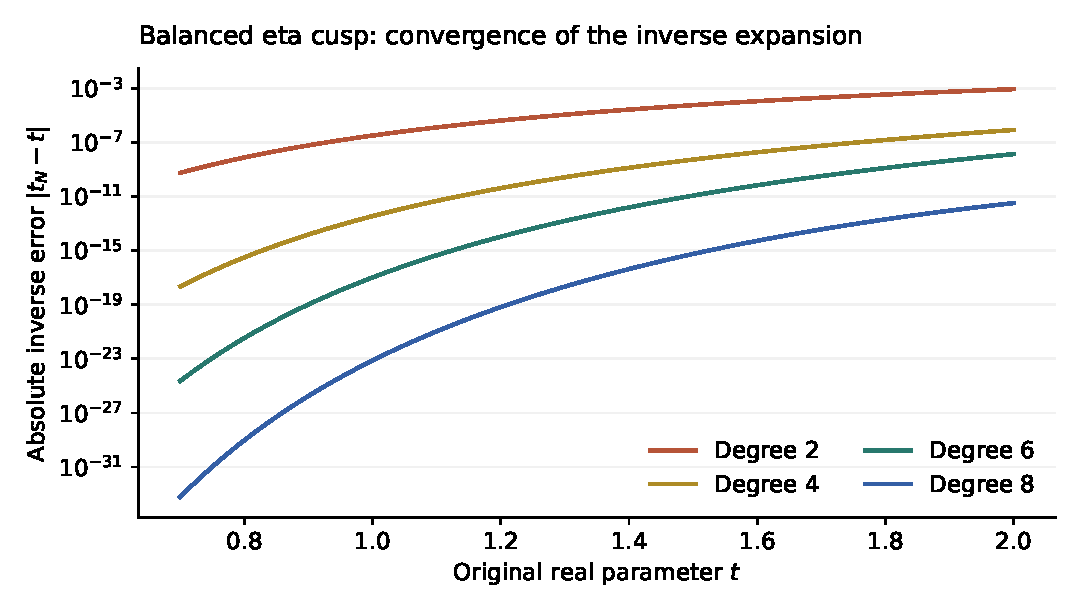
\includegraphics[width=.96\textwidth]{figures/eta_inverse_convergence.pdf}
 \caption{Observed error after truncating the nome inverse \(Q(s)\)
 at degrees \(2,4,6,8\), then taking a coherent logarithm.
 Each curve uses direct high precision evaluation of the eta example.
 Moving toward the cusp makes the exponential coordinate smaller.
 The curves are numerical illustrations; the analytic tail bounds
 are \cref{eq:flat-certified,eq:product-tail}.}
 \label{fig:convergence}
\end{figure}

The archive also records the rational \(q\)-gamma product
checks for \(k=2,3,4\), the four-factor family at real and
complex arguments, explicit rational-cusp phase checks, and
paired-term Stokes contour checks.
The latter compare the two directional integrals with their
residue sum; the counterexample itself is established by its
contour proof, independently of those calculations.

The supplementary phase program checks 24 one-factor and 24
general-product identities, with both real and complex parameters,
at 80 decimal digits.  The largest scaled residual is less than
\(1.3\times10^{-79}\).  It also checks Dedekind reciprocity with
exact rational arithmetic and records the rational certificate in
\cref{eq:explicit-H-bound}.
The Stokes program independently integrates four paired summands
along the two rays; each difference agrees with its residue sum to
absolute error less than \(4\times10^{-82}\).
These are reproducible checks at specified working precision;
the numerical residuals are not interval-arithmetic certificates.

\subsection{An implementation procedure}

A reliable implementation can follow this sequence.
\begin{enumerate}[leftmargin=*,itemsep=3pt]
\item Record the input function, variable being inverted, cusp,
      target normalization, sector, and logarithm lift.
\item For a finite eta or Euler quotient, compute
      \(g_d,\rho_d,A_{h,k},B,D\) exactly.
      Select the appropriate core regime.
\item Combine coincident action coefficients in a cyclotomic
      field before identifying the first surviving term.
\item Use the exact-core theorem, the finite-endpoint scale,
      or the flat-cusp inverse according to that regime.
      Near a zero of the core derivative, change the local chart.
\item Generate coefficients to the desired order, verify
      composition algebraically, and compute a disk or tail bound.
\item Evaluate products through the dual nome, preserving
      logarithm lifts.  If the target comes from a Borel sum,
      carry the contour's residue correction into the equation.
\end{enumerate}

This procedure makes two common failure modes explicit.
Deleting a flat modular factor may remove the entire inverse
problem after balancing.  Ignoring a Stokes correction may
invert a different sectorial function while preserving the same
formal power series.

\section{Further research questions and precise remaining boundaries}
\label{sec:future}

The article supplies exact results for substantial classes, but a
general complex transseries program has additional problems.
The following questions separate those problems by the missing
mathematical ingredient.

\begin{question}[Uniform parameter-dependent resurgent inversion]
Starting with \cref{eq:cb-borel}, prove the full family of
resurgent seminorm bounds needed for implicit inversion in
\(a\), uniformly on compact subsets of \(|a|<1\), with specified
contours and target jumps.  Identify a natural function space in
which both the contour correction and the inverse depend
holomorphically on the parameters.
\end{question}

The meromorphic Borel transform and the exact equation
\cref{eq:cb-inverse-exact} are available.
A pointwise nonzero derivative does not by itself supply uniform
inverse radii or all of the needed functional analytic estimates.
This is the part of the repository's implicit conjecture that
has not been replaced here by an unconditional general theorem.

\begin{question}[Coalescing fixed-argument and modular limits]
Obtain a uniform inverse theory when \(a=a(t)\) approaches the
unit circle, for example \(a(t)=\ee^{-\alpha t}\), while
\(q=\zeta\ee^{-t}\to\zeta\).
How do the Borel pole arrays reorganize into the modular
completions when \(\alpha\) is rational, and what replaces those
completions for general complex \(\alpha\)?
\end{question}

The fixed compact-\(a\) estimates deteriorate as \(|a|\to1\).
The exact eta and rational \(q\)-gamma identities avoid that
deterioration in special cases but do not prove a uniform
transition theorem for arbitrary \(\alpha\).
A useful first goal is a two-parameter sector with an explicit
matching estimate on an overlap.

\begin{question}[Moving cusps with growing denominator]
For fixed dilations and rational cusps \(h/k\) depending on \(t\),
determine uniform reversion and error bounds across the
transition \(k^2t\asymp1\), including the phase arithmetic.
\end{question}

The exact normal form remains valid.
What fails is the conclusion \(Q\to0\).
A transition approximation must retain a non-small dual product,
and cannot follow from a finite number of its coefficients.
Uniform control in \(h\) and \(k\) is a separate issue from
the fixed-cusp formula.

\begin{question}[Effective cancellation certificates]
Given a finite phase Euler product, find practical bounds on
the first nonzero coefficient of its logarithm, or prove that
it is identically zero.
Can modular-form bounds and arithmetic coefficient recurrences
be combined to outperform direct expansion, including products
with nontrivial eta multipliers?
\end{question}

The constructions here have visible first coefficients.
For arbitrary phase products, cancellation can be extensive or
complete.  An effective certificate should also identify the
primitive action lattice, so that a reported ramification
order is intrinsic to the chosen minimal nome.

\begin{question}[Optimal level and height for a prescribed ramification]
Among all balanced products realizing order \(m\), minimize
the common level, the largest original dilation, or the sum of
the absolute exponents.  Determine the tradeoff between those
quantities under two versus three balance constraints.
\end{question}

The factor counts three and four are sharp.
They do not optimize the level of the four-factor construction,
which uses an lcm of four consecutive integers.
The one-dimensional classification
\cref{eq:four-support-classification} supplies an exact starting
point for the optimization.

\begin{question}[Global continuation and coefficient asymptotics]
For a specific balanced quotient, locate the first singularities
of \(\Psi(u)\), including critical values of the dual product
and images of other cusps.  Determine the exact convergence
radius and the large-order asymptotics of its inverse coefficients.
\end{question}

The local inverse theorem gives a positive radius, not its
optimal value.  Modular coordinates may permit a global analysis
in low-level examples.  Such an analysis requires a verified
description of the relevant modular curve or covering and should
not be inferred from a few inverse coefficients.

\begin{question}[Unfolding a flat critical point]
Let a parameter break one or more balance equations, so that
\[
 F_\varepsilon(t)=
 C\,t^{-b(\varepsilon)}
 \ee^{-a(\varepsilon)/t+c(\varepsilon)t}
 R_\varepsilon(\ee^{-S/t}).
\]
Construct uniform inverse charts as the algebraic core and the
flat defect become comparable.
\end{question}

Theorems for each separate regime do not automatically remain
uniform when \(a,b,c\to0\).
Natural transition variables compare
\(a/t\), \(b\log t\), and \(ct\) with
the first surviving \(Q\)-action.
This is a singular perturbation problem rather than an ordinary
fixed-parameter application of the inverse-function theorem.

\begin{question}[Finite moving critical points and higher multiplicity]
Extend the present exact examples to a parameter-dependent
critical point of multiplicity \(m\), with explicit moving
discriminants, sheet radii, and crossover bounds.
\end{question}

The generic local Puiseux theorem is already available in the
repository.  A perturbed critical point may split.
For instance \(u^2+\varepsilon u=y\) has its critical value at
\(-\varepsilon^2/4\), so an expansion about the undeformed
critical value is not uniform.
The arbitrary-\(m\) cusp constructions do not solve that
full moving-discriminant problem.

\begin{question}[Infinite and accumulating complex actions]
Replace the finite analytic action set by a countable one,
possibly with accumulation in exponential height.
Find conditions under which coefficient grouping, analytic
substitution, and inverse summation remain compatible.
\end{question}

The finite decay-cone argument bounds the number of indices at
each height.  It does not extend merely by writing an infinite
list of actions.  A viable theorem needs quantitative summability
of grouped coefficients and control of the inverse iteration.

\begin{question}[More \(q\)-special functions and joint criticality]
Determine which rational combinations of \(q\)-beta,
\(q\)-gamma, \(q\)-Barnes functions, and Gaussian coefficients
admit exact modular completions with enough balance to create
flat critical values.  Study joint argument/base critical limits.
\end{question}

The product identities in \cref{sec:qgamma} provide a
testable model: first isolate an exact analytic background, then
identify the surviving modular coordinate and apply the
appropriate inverse theorem.
Existing questions on optimal \(q\)-multinomial truncation,
pole pinching, and the motion of the \(q\)-gamma minimum remain
distinct \cite{repo-qsharp,repo-qmono}.

\begin{question}[Formal verification of the analytic boundary]
Formalize the finite arithmetic recurrences and balance
constructions, then connect them to a verified analytic
inverse theorem and explicit complex product bounds.
\end{question}

The rational coefficient generator is a suitable first target.
A full proof also needs complex branch data, normal convergence,
Rouch\'e or contraction certificates, and the modular identity.
No theorem in this article is claimed to have been checked by
a proof-assistant kernel.  The included programs check exact
finite algebra and numerical examples.

\subsection{What is settled here}

The directional-equality assertion in the named repository
conjecture has an explicit counterexample, while its
fixed-argument Gevrey and Borel-continuation content has a
direct, literature-consistent proof.
The complete-cancellation question has explicit arbitrary-order
examples with sharp factor counts.
The inverse charts have all coefficients, all small-nome
logarithmic sheets, and quantitative tails.
The rational \(q\)-gamma applications distinguish the flat
normalized inverse from the regular-core inverse of the original
observable.

These conclusions are compatible with the limits stated
throughout: fixed sectors and branches are part of the data;
a fixed-cusp formula is not a growing-denominator theorem;
local convergence is not global continuation; and a finite
analytic action model is not the entire field of complex
transseries.

\clearpage
\begin{thebibliography}{99}
\addcontentsline{toc}{section}{References}

\bibitem{vdh-book}
Joris van der Hoeven,
\emph{Transseries and Real Differential Algebra},
Lecture Notes in Mathematics 1888, Springer, 2006.
Sections 5.4 and 6.5.
\url{https://www.texmacs.org/joris/ln/ln.html}.

\bibitem{vdh-complex}
Joris van der Hoeven,
\emph{Complex transseries solutions to algebraic differential equations},
author's online version, 2001.
Especially Section 2.7 on composition.
\url{https://www.texmacs.org/joris/osc/osc.html}.

\bibitem{edgar}
Gerald A. Edgar,
\emph{Transseries: Composition, Recursion, and Convergence},
arXiv:0909.1259, 2009.
\url{https://arxiv.org/abs/0909.1259}.

\bibitem{sauzin}
David Sauzin,
Nonlinear analysis with resurgent functions,
\emph{Annales scientifiques de l'\'Ecole Normale Sup\'erieure}
\textbf{48} (2015), 667--702.
\url{https://doi.org/10.24033/asens.2255}.
Preprint: \url{https://arxiv.org/abs/1212.4477}.

\bibitem{marmi-sauzin}
Stefano Marmi and David Sauzin,
\emph{Quasianalytic monogenic solutions of a cohomological equation},
Memoirs of the American Mathematical Society
\textbf{164} (2003), no.~780.
\url{https://doi.org/10.1090/memo/0780}.
Preprint: \url{https://arxiv.org/abs/math/0101149}.

\bibitem{garoufalidis-kashaev}
Stavros Garoufalidis and Rinat Kashaev,
Resurgence of Faddeev's quantum dilogarithm,
\emph{IRMA Lectures in Mathematics and Theoretical Physics}
\textbf{33} (2021), 257--272.
\url{https://doi.org/10.4171/IRMA/33-1/14}.
Preprint: \url{https://arxiv.org/abs/2008.12465}.

\bibitem{fantini-rella}
Veronica Fantini and Claudia Rella,
Modular resurgence, \(q\)-Pochhammer symbols, and quantum operators
from mirror curves,
\emph{Letters in Mathematical Physics} \textbf{116} (2026), article 39.
\url{https://doi.org/10.1007/s11005-026-02063-x}.
\url{https://arxiv.org/abs/2506.08265}.

\bibitem{kong-teo}
Ze-Yong Kong and Lee-Peng Teo,
\emph{An Elementary Proof of the Transformation Formula for the
Dedekind Eta Function},
arXiv:2302.03280, 2023.
\url{https://arxiv.org/abs/2302.03280}.

\bibitem{dlmf-eta}
NIST Digital Library of Mathematical Functions,
Section 23.18, \emph{Modular Transformations},
especially equations 23.18.5--23.18.7.
\url{https://dlmf.nist.gov/23.18}.
Accessed 4 October 2026.

\bibitem{dlmf-qgamma}
NIST Digital Library of Mathematical Functions,
Section 5.18, \emph{\(q\)-Gamma and \(q\)-Beta Functions}.
\url{https://dlmf.nist.gov/5.18}.
Accessed 4 October 2026.

\bibitem{dlmf-theta}
NIST Digital Library of Mathematical Functions,
Sections 20.2 and 20.5, theta-function series and products,
especially equation 20.5.4.
\url{https://dlmf.nist.gov/20.2};
\url{https://dlmf.nist.gov/20.5}.
Accessed 4 October 2026.

\bibitem{repo-trans}
VladimirReshetnikov/\repo{},
\emph{Transseries: the polynomial--logarithmic calculus, series reversal
at infinity, and the inversion of rapidly growing functions}.
Canonical volume and group documentation in
\texttt{Analysis/Transseries/docs/series-and-transseries/}.
Inspected snapshot:
\texttt{6cb1d86f19ebf9f54c8d985b141b84233b6eab66}.
\href{https://github.com/VladimirReshetnikov/ProveIt/blob/6cb1d86f19ebf9f54c8d985b141b84233b6eab66/Analysis/Transseries/docs/series-and-transseries/README.md}{Pinned group README}.

\bibitem{repo-companion}
VladimirReshetnikov/\repo{},
\emph{Combinatorial Transseries and Their Inverses:
Gamma quotients, finite exponential sums, moment sectors,
moving saddles, arithmetic sheets, and \(q\)-products}.
Pinned source as in \cite{repo-trans};
especially labels \texttt{t3:eq:modularP} and
\texttt{t3:eq:modularsectors}.
\href{https://github.com/VladimirReshetnikov/ProveIt/blob/6cb1d86f19ebf9f54c8d985b141b84233b6eab66/Analysis/Transseries/docs/series-and-transseries/Combinatorial_Transseries_Inverses/Combinatorial_Transseries_Inverses.tex}{Pinned companion source}.

\bibitem{repo-reversion}
VladimirReshetnikov/\repo{},
\emph{Support-Controlled Reversion and the Exact One-Exponential
Substitution Class}.
Pinned source as in \cite{repo-trans}; especially the research
questions on several actions and analytic subclasses.
\href{https://github.com/VladimirReshetnikov/ProveIt/blob/6cb1d86f19ebf9f54c8d985b141b84233b6eab66/Analysis/Transseries/docs/series-and-transseries/Support_Controlled_Reversion_One_Exponential/reversion_and_one_exponential.tex}{Pinned reversion source}.

\bibitem{repo-fold}
VladimirReshetnikov/\repo{},
\emph{Critical Transseries at a Moving Fold}.
Pinned source as in \cite{repo-trans}; labels
\texttt{thm:atlas}, \texttt{thm:actions}, and \texttt{thm:grid}.
\href{https://github.com/VladimirReshetnikov/ProveIt/blob/6cb1d86f19ebf9f54c8d985b141b84233b6eab66/Analysis/Transseries/docs/series-and-transseries/Critical_Transseries_Moving_Fold/article.tex}{Pinned moving-fold source}.

\bibitem{repo-qmono}
VladimirReshetnikov/\repo{},
\(q\)-Pochhammer and \(q\)-binomial monograph,
in the Fabius-function \texttt{exponents-and-q-series} research
directory.  Pinned snapshot as in \cite{repo-trans}.
Chapters 1, 3, and 5; labels
\texttt{thm:uq-finite-ramification},
\texttt{thm:ip-fixed-a-inverse},
\texttt{thm:ip-eta-completions},
\texttt{thm:ip-radial-cyclotomic},
and \texttt{thm:qs-qgamma-one}.
\href{https://github.com/VladimirReshetnikov/ProveIt/blob/6cb1d86f19ebf9f54c8d985b141b84233b6eab66/Analysis/FabiusFunction/docs/semi-formalized-research-frontiers/drafts/exponents-and-q-series/q_pochhammer_q_binomial_monograph/chapters/03_infinite_q_pochhammer.tex}{Pinned chapter 3};
\href{https://github.com/VladimirReshetnikov/ProveIt/blob/6cb1d86f19ebf9f54c8d985b141b84233b6eab66/Analysis/FabiusFunction/docs/semi-formalized-research-frontiers/drafts/exponents-and-q-series/q_pochhammer_q_binomial_monograph/chapters/05_q_special_functions.tex}{pinned chapter 5}.

\bibitem{repo-qfrontier}
VladimirReshetnikov/\repo{},
\(q\)-Pochhammer and \(q\)-binomial monograph,
Chapter 7, \emph{Certification and frontiers}.
Pinned snapshot as in \cite{repo-trans};
conjecture \texttt{conj:cyclotomic-resurgent-inverse}.
\href{https://github.com/VladimirReshetnikov/ProveIt/blob/6cb1d86f19ebf9f54c8d985b141b84233b6eab66/Analysis/FabiusFunction/docs/semi-formalized-research-frontiers/drafts/exponents-and-q-series/q_pochhammer_q_binomial_monograph/chapters/07_certification_and_frontiers.tex}{Pinned conjecture source}.

\bibitem{repo-qsharp}
VladimirReshetnikov/\repo{},
\emph{Uniform \(q\)-Multinomial Transseries and Certified Inversion},
\emph{Theta-Resolved Optimal Truncation of \(q\)-Multinomial
Transseries}, and
\emph{Uniform Resurgent Crossover for Gaussian Binomials}.
Pinned snapshot as in \cite{repo-trans}; future questions on
complex sectors, pole pinching, root-of-unity crossover, and
modular normalization.
\href{https://github.com/VladimirReshetnikov/ProveIt/blob/6cb1d86f19ebf9f54c8d985b141b84233b6eab66/Analysis/Transseries/docs/series-and-transseries/Uniform_q_Multinomial_Certified_Inversion/uniform_q_multinomial_transseries.tex}{Pinned \(q\)-multinomial source};
\href{https://github.com/VladimirReshetnikov/ProveIt/blob/6cb1d86f19ebf9f54c8d985b141b84233b6eab66/Analysis/Transseries/docs/series-and-transseries/Theta_Resolved_Optimal_Truncation_q_Multinomial/article.tex}{pinned theta-truncation source}.

\end{thebibliography}


\end{document}
